\documentclass[twocolumn]{aastex701}
\usepackage{amsmath,amssymb}
\usepackage{minted}
\usepackage{xcolor}
\hypersetup{colorlinks=true,linkcolor=linkcolor,citecolor=linkcolor,urlcolor=linkcolor}
\definecolor{linkcolor}{rgb}{0,0,0.25}
\usemintedstyle{friendly}
% Macros; conventions follow the galpy paper (Bovy 2015, ms.in)
\setlength{\emergencystretch}{5em}
\allowdisplaybreaks
\raggedbottom
\newcommand{\ie}{i.e.}
\newcommand{\eg}{e.g.}
\newcommand{\etal}{et al.}
\newcommand{\dd}{\mathrm{d}}
\newcommand{\sectionname}{$\mathsection$}
\newcommand{\figurenames}{\figurename s}
\newcommand{\eqnname}{equation}
\newcommand{\Eqnname}{Equation}
\newcommand{\equationname}{\eqnname}
\renewcommand{\vec}[1]{\ensuremath{\mathbf{#1}}}
\newcommand{\unitvec}[1]{\ensuremath{\mathbf{\hat{#1}}}}
\newcommand{\vecx}{\ensuremath{\vec{x}}}
\newcommand{\vecv}{\ensuremath{\vec{v}}}
\newcommand{\vecw}{\ensuremath{\vec{w}}}
\newcommand{\vecj}{\ensuremath{\vec{J}}}
\newcommand{\veco}{\ensuremath{\vec{\Omega}}}
\newcommand{\veca}{\ensuremath{\boldsymbol\theta}}
\newcommand{\paramspot}{\ensuremath{\vec{p}}}
\newcommand{\inv}{\ensuremath{^{-1}}}
\newcommand{\kpc}{\ensuremath{\,\mathrm{kpc}}}
\newcommand{\pc}{\ensuremath{\,\mathrm{pc}}}
\newcommand{\kms}{\ensuremath{\,\mathrm{km\ s}^{-1}}}
\newcommand{\Gyr}{\ensuremath{\,\mathrm{Gyr}}}
\newcommand{\Myr}{\ensuremath{\,\mathrm{Myr}}}
\newcommand{\yr}{\ensuremath{\,\mathrm{yr}}}
\newcommand{\msun}{\ensuremath{\,\mathrm{M}_{\odot}}}
\newcommand{\mas}{\ensuremath{\,\mathrm{mas}}}
% code names
\newcommand{\flag}[1]{\texttt{#1}}
\newcommand{\galpy}{\flag{galpy}}
\newcommand{\numpy}{\flag{numpy}}
\newcommand{\scipy}{\flag{scipy}}
\newcommand{\matplotlib}{\flag{matplotlib}}
\newcommand{\astropy}{\flag{astropy}}
\newcommand{\jax}{\flag{jax}}
\newcommand{\torch}{\flag{PyTorch}}
\newcommand{\python}{\flag{Python}}
\newcommand{\cc}{\texttt{C}}
\newcommand{\diffrax}{\flag{diffrax}}
\newcommand{\torchode}{\flag{torchode}}
\newcommand{\git}{\texttt{git}}
\newcommand{\github}{\texttt{GitHub}}
\newcommand{\pot}{\texttt{Potential}}
\newcommand{\orb}{\texttt{Orbit}}
\newcommand{\claude}{Claude}
% code listings: inline snippets use \begin{minted}{python}; listings shown as
% numbered figures use the galpy-paper options below
\newminted{python}{fontsize=\small,autogobble,breaklines}
\newenvironment{code}{\VerbatimEnvironment\begin{pythoncode}}{\end{pythoncode}}
\newenvironment{codefig}{\VerbatimEnvironment\begin{minted}[mathescape,linenos,numbersep=5pt,autogobble,frame=lines,framesep=2mm,fontsize=\small]{python}}{\end{minted}}
\newcommand{\pycode}[1]{\mintinline{python}{#1}}

\shorttitle{galpy with jax and PyTorch backends}
\shortauthors{Bovy}

\begin{document}

\title{\galpy\ with differentiable, accelerated backends: galactic dynamics in \jax\ and \torch}

\author[0000-0001-6855-442X]{Jo Bovy}
\affiliation{David A. Dunlap Department of Astronomy and Astrophysics, University of Toronto, 50 St.~George Street, Toronto, ON M5S 3H4, Canada}
\email{bovy@astro.utoronto.ca}

\begin{abstract}
We describe an extension of \galpy, the \python\ library for galactic
dynamics, that adds \jax\ and \torch\ as computational backends
alongside its existing \numpy\ and \cc\ implementation. With it,
\galpy's gravitational potentials, orbit integration, action--angle
transformations and their inverses, and distribution functions,
including those for tidal streams, run on GPUs, can be compiled as part
of a user's program, and can be differentiated with respect to their
inputs and parameters, from the force at a point to the samples drawn
from a distribution function. The user-facing design is kept simple: the
active backend follows from the type of the arrays that are passed in,
the \galpy\ interface is unchanged, and the \numpy\ path gives the same
results as before. We describe the design of the
backend framework and its implementation in each of \galpy's modules,
with examples of use, and we discuss its limitations. On a GPU, batches
of orbits, samples from distribution functions, and stream models run
one to five orders of magnitude faster than on a single CPU core. To
illustrate the new capabilities, we present simple examples of fitting
the Galactic potential with a hypervelocity star and of learning the
inverse action--angle transformation with a neural network trained
through \galpy. An AI coding agent wrote
essentially all of the code under the detailed direction and review of
the human author, and we describe how we organized this work and how we
established the correctness of the result. This work is the start of
\galpy's version~2, which is available at
\url{https://github.com/jobovy/galpy} and documented at
\url{https://docs.galpy.org/en/v2/}.

\end{abstract}

\keywords{\uat{Galaxy dynamics}{591} --- \uat{Stellar dynamics}{1596} --- \uat{Milky Way dynamics}{1051} --- \uat{Stellar streams}{2166} --- \uat{Astronomy software}{1855} --- \uat{Computational methods}{1965}}

\section{Introduction}\label{sec:intro}

Software for galactic dynamics has become a standard part of the toolkit
of Galactic astronomy. Codes such as the NEMO Stellar Dynamics Toolbox
\citep{Teuben1995}, \galpy\ \citep{Bovy2015}, \texttt{gala}
\citep{PriceWhelan2017}, and \texttt{AGAMA} \citep{Vasiliev2019}
provide gravitational potentials, orbit integration, action--angle
coordinates, and distribution functions (DFs) in a form that can be
applied directly to observed stars, and they are used both to place
individual objects on their orbits and to build dynamical models that
are fit to data. The reason that such codes are useful is simple: the
motion of a star in a given gravitational potential is a solved
problem, but one that requires careful numerical work, and a
well-tested implementation that is shared saves every user from
repeating that work and from the mistakes made along the way. The
kinematic data from the Gaia mission
\citep{Gaia2016,Gaia2018,Gaia2023}
have made such codes indispensable, because for the first time orbits
can be computed for hundreds of millions of stars.

\citet{Bovy2015} introduced \galpy\ as a \python\ package, with \cc\
implementations of the time-critical parts, for computing orbits,
action--angle coordinates, and DFs in general galactic potentials. It has
since been used in more than a thousand papers (1,056 at the time of
writing, from four in 2012 to about 170 per year since 2024). Most of
these use \galpy\ as a tool: orbits are integrated in a model of the
Milky Way to place objects in the Galaxy and to characterize their
motion. In this way, \galpy\ has been applied to stars in the disk with
measured abundances and ages \citep[\eg,][]{Frankel2020,Xiang2022},
to the substructure of the stellar halo \citep[\eg,][]{Belokurov2020,
Lane2023}, to globular clusters and dwarf galaxies \citep[\eg,][]{Fritz2018,
Pace2022}, to hypervelocity and runaway stars and to the natal kicks of
pulsars and compact objects \citep[\eg,][]{Boubert2018,Marchetti2022,
ODoherty2023}, to open clusters and the star-forming regions near the
Sun \citep[\eg,][]{Zucker2022,Swiggum2024}, to the hosts of exoplanets
and to interstellar objects \citep[\eg,][]{Stefansson2023,Forbes2025},
and to galaxies other than our own \citep[\eg,][]{Tonnesen2019}. A
smaller set of papers, perhaps one in six, uses \galpy\ as a modeling
framework in which a DF or a potential is fit to data: models of tidal
streams and of their perturbations by dark-matter subhalos
\citep[\eg,][]{Bovy2016,Malhan2019,Banik2021}, action-based models of
the disk \citep[\eg,][]{Trick2016,Mackereth2019}, DF and Jeans models
of the halo \citep[\eg,][]{Lane2023}, models of the Galactic bar
\citep[\eg,][]{Hunt2018,Lucey2023}, and measurements of the Milky Way's
mass and potential \citep[\eg,][]{Cautun2020}. It is for this second
kind of use that derivatives matter, because fitting a model to data
requires the likelihood to be evaluated many times over the model's
parameters, and the efficiency of this search is set by whether its
derivatives are available.

\galpy\ has changed much since 2015, but the trends are simple to
state. The number of potentials grew from 22 to 72, with the growth
shifting from specific density profiles to general solvers (basis-function,
multipole, and interpolated potentials) and to wrappers that make any
potential time-dependent, rotating, or tilted, and \galpy\ gained
dissipative forces, such as dynamical friction, and non-inertial
reference frames. The
\orb\ class was rewritten as an arbitrarily-shaped array of orbits that
are integrated in parallel, such that millions of orbits can be handled
at once. DFs for tidal streams were extended to stream gaps
\citep{Sanders2016} and to particle-spray models \citep{Fardal2015,
Chen2025}, and a general framework for spherical DFs appeared. The
action--angle module gained inverse transformations and the orbit module
gained chaos diagnostics, surfaces of section and Lyapunov exponents. In
2026, we implemented the three-dimensional variational equations that
propagate the derivatives of an orbit with respect to its initial
conditions in \cc\ for most of the potential library. Over the same
period the code grew from 36,000 to 93,000 lines of \python\ and from
8,000 to 26,000 lines of \cc, and the test suite grew from 500 to 2,300
tests that cover all of the code.

Over the same decade, numerical computing has been reshaped by
frameworks built for machine learning, chiefly \jax\
\citep{Bradbury2018} and \torch\ \citep{Paszke2019}. These provide
array programming that runs on CPUs and GPUs alike, just-in-time
compilation of whole programs, and automatic differentiation (AD) of
arbitrary code \citep[see][for a review]{Baydin2018}. A dynamics code
written in such a framework gains three things: it runs on a GPU, where
large batches of orbits or stars are processed at once; it can be
compiled into a single program rather than executed one array operation
at a time; and every quantity that it computes---a force, an orbit, an
action, the value of a DF---can be differentiated with respect to every
input, be it an initial condition or a parameter of the potential.
Derivatives are what gradient-based inference requires, whether this is
Hamiltonian Monte Carlo \citep{Duane1987,HoffmanGelman2014}, variational
inference, or the optimization of models with many parameters, such as
neural networks that stand in for a potential or a DF. Codes built on
these frameworks are now in use in cosmology
\citep[\eg,][]{Modi2021,Campagne2023,Li2024} and, over the past two
years, in galactic dynamics. \texttt{galax} \citep{Starkman2026}, a
\jax\ code modeled on \texttt{gala}, provides the halo potentials whose
acceleration directions are compared with the curvature of stellar
streams around other galaxies to constrain the shapes of their halos
\citep{Wu2026b,Euclid2026}, and the orbits used to forecast how well
such curvature tests separate dark-matter models \citep{Starkman2026b}.
\citet{AnauMontel2026} integrate streams perturbed by subhalos with
\texttt{galax} on a GPU and obtain Fisher forecasts by differentiating
the full simulation. Other \jax\ codes fit the progenitor and the host
potential of a mock stream by gradient descent through an $N$-body
simulation \citep{Viterbo2025}, generate the many particle-spray models
needed to infer the distribution of halo flattenings from a population
of streams \citep{Chemaly2026}, and compute the response of streams to
subhalos by integrating linearized equations of motion
\citep{Nibauer2025}. Gradient-based samplers in \jax\ fit a spline
model of the track of GD-1 to measure the accelerations along it
\citep{Nibauer2025b}, and a flexible model of vertical orbits to the
variation of stellar abundances \citep{PriceWhelan2025}. Normalizing
flows for the DF, differentiated automatically, recover the potential
from phase-space snapshots of simulated galaxies
\citep{Green2023,An2021,Buckley2023} and of 5.6 million \textit{Gaia}
stars \citep{Kalda2025}. Differentiating an entire simulation
\citep{Viterbo2025,AnauMontel2026}, or fitting a neural-network
potential to millions of stars \citep{Kalda2025}, is not practical with
codes that only return values.

In this paper, we describe an extension of \galpy\ that adds \jax\ and
\torch\ as \emph{backends} to its existing \numpy\ and \cc\
implementation. The principle that guided this work is that nothing
should change for the existing user: the \numpy\ path produces results
that are byte-for-byte identical to those of the previous version, the
interface is unchanged, and \galpy's existing test suite now runs under
every backend, in eager and in compiled mode, with the same tolerances.
Backends are selected by the type of the arrays that are passed in or
through a context manager; \galpy's code is written against a
backend-agnostic array namespace; and \galpy\ does not compile anything
itself, but is written such that it can be compiled and differentiated
as part of the user's own program. Most of \galpy\ is covered: the
potentials and their forces and derivatives, orbit integration either
inside the backend or through the \cc\ integrators with their variational
equations, the action--angle transformations and their inverses, and the
DFs, including those for tidal streams. All of these are differentiable
with respect to their inputs and parameters, and they run on GPUs. We
list what is not covered where it comes up; the main gaps are the
torus-mapping code and the use of \astropy\ units inside compiled
programs.

Claude, an AI coding agent developed by Anthropic, wrote essentially all
of the code described in this paper, working in the \texttt{Claude Code}
environment under the direction and review of the human author (JB)
between June and October 2026. We discuss how this was done, how we
organized the work, and how we established the correctness of the code
in \sectionname~\ref{sec:process}; a statement on the use of AI, which
also explains the use of ``we'' in a paper with a single human author,
appears at the end of the paper.

The outline of this paper is as follows. \sectionname~\ref{sec:design}
describes the design of the backend framework: how a backend is chosen,
how we made \galpy's code backend-agnostic, the utilities that this
required, and how we made the test suite run under every backend. The
following sections go through \galpy's main modules in turn: potentials
in \sectionname~\ref{sec:potential}, orbit integration and its derivatives
in \sectionname~\ref{sec:orbit}, action--angle coordinates in
\sectionname~\ref{sec:aa}, DFs in \sectionname~\ref{sec:df}, and models
of tidal streams in \sectionname~\ref{sec:streams}. Each of these
sections starts from the general approach and then gives the details that
are specific to the module, with examples of use. \sectionname~\ref{sec:process}
describes the development process. \sectionname~\ref{sec:examples}
presents fuller examples that combine several parts of the code in a
single analysis, and \sectionname~\ref{sec:conclusion} concludes. An
Appendix gives the variational equations behind the orbit derivatives.

Code to reproduce all of the figures in this paper, as well as the
working notes of the development, is available in a \git\ repository
associated with this paper, separate from the \galpy\ repository, at
\\ \centerline{\url{https://github.com/jobovy/galpy-jax}~.}

\section{Design of the backend framework}\label{sec:design}

\subsection{Principles}\label{sec:design-principles}

Six rules were fixed before any code was written, and the rest of this
paper is largely a description of how they were kept. First, the
\numpy\ path is byte-identical to the previous version of \galpy. Every
backend helper is a strict pass-through when the active array library is
\numpy, such that migrated code written as \texttt{xp.sqrt(x)}, where
\texttt{xp} is the resolved namespace, runs the identical \numpy\ function
on the identical object. This rule is enforced by tests and, for each
PR, by comparing checksums of outputs between a checkout with and one
without the change. Where the \numpy\ result did change, this was
flagged and approved; there are three such places, discussed where they
arise. Second, the interface is unchanged: the same classes, methods,
and keywords, with the backend determined by the arrays that are passed
in. Third, \galpy's code is written against a backend-agnostic array
namespace, with backend-specific code confined to the \texttt{galpy.backend}
subpackage and never written as \texttt{if backend == 'jax'} inside the
physics. Fourth, \galpy\ uses the basic array operations of \jax\ and
\torch\ and little else; the numerical methods that \scipy\ supplies on
the \numpy\ path---special functions, root finding, quadrature,
interpolation, sampling---are implemented in \texttt{galpy.backend} and
tested against \scipy\ and against arbitrary-precision references,
rather than taken from the frameworks' own, uneven, \scipy-like
modules. Fifth, \galpy\ never compiles anything itself: the code is
written to be traceable by \texttt{jax.jit} and \texttt{torch.compile},
and the user decides what to compile. Sixth, the existing test suite,
run under every backend with the same tolerances, is the acceptance
test.

\subsection{Choosing a backend}\label{sec:design-choosing}

The backend follows the data. A \galpy\ function that receives a \jax\
array or a \torch\ tensor computes with that framework and returns an
array of the same kind; a function that receives \numpy\ arrays or
\python\ scalars computes with \numpy\ as before. Thus, the radial force
of the standard Milky-Way model is evaluated on a \jax\ array as
\begin{code}
from galpy.potential import MWPotential2014, evaluateRforces
R= jnp.linspace(0.5,2.,1001)
FR= evaluateRforces(MWPotential2014,R,0.) # a jax array, on R's device
\end{code}
without any further instruction, and with a \torch\ tensor the same
call returns a tensor. When there is no array to dispatch on, as when
a user sets up an \orb\ instance from \python\ floats, the default
backend is used; it is \numpy\ unless a different one is set in the
configuration file or through a context manager,
\begin{code}
import galpy.backend
with galpy.backend.use('jax'):
    o= Orbit([1.,0.1,1.1,0.,0.05,0.]) # initial condition becomes a jax array
    o.integrate(ts,MWPotential2014)   # ... and the orbit is integrated in jax
\end{code}
The resolution order is therefore: an explicit \texttt{xp=} argument,
the array arguments, the context or configured default, and finally
\numpy. The context manager also accepts \texttt{force=True}, which makes
the default take precedence over the data; this is what the test suite
uses to run \galpy's existing tests, written with \numpy\ inputs, under
a different backend, and it is not meant for production code.

Backend arrays go in and come out, but a few conventions are needed at
the edges. \galpy\ computes in double precision, and its internal
constants are \python\ floats, such that under \torch, whose default
is single precision, \galpy\ enters a double-precision default for the
duration of a call; a user's single-precision tensor stays single
precision in and out. Outputs that are scalars in the \numpy\ sense,
such as a single potential value for scalar inputs under a forced
backend, are returned as \numpy\ values, because \astropy\ units cannot
wrap a backend array. Units are handled outside the backend layer: a
\texttt{Quantity} input is converted to \galpy's internal units by the
existing unit-handling decorators before it reaches the backend code,
and a \texttt{Quantity} output is built from the result afterwards. A
potential parameter that is given as a backend array carries no units
and is taken to be in internal units already; this is what makes it
possible to differentiate with respect to it. \texttt{Quantity} objects
cannot be traced by \texttt{jax.jit}, and the use of units inside a
compiled program is therefore not supported (this accounts for three of
the six tests that remain in the ledger of
\sectionname~\ref{sec:process-ledger}).

\subsection{Backend-agnostic code}\label{sec:design-agnostic}

Every migrated compute method starts by resolving the array namespace
from its coordinate arguments and then uses only that namespace,
\begin{code}
def _evaluate(self,R,z,phi=0.,t=0.):
    xp= get_namespace(R,z,phi,t)
    return -self._amp/xp.sqrt(R**2+z**2+self._b2)
\end{code}
The namespace is the plain \numpy\ module for \numpy\ data,
\texttt{jax.numpy} for \jax\ arrays, and the array-API-compatible view of
\torch\ for tensors, obtained through the \texttt{array-api-compat}
package. This is the entire change for the majority of \galpy's
potentials, which are elementary functions of the coordinates; the
work is in the remainder, where \scipy\ or \numpy-specific functions
were used, and that work is described in the module sections. The
dispatch costs about $3\,\mu$s per call when run eagerly and nothing
under compilation, where it is resolved at trace time.

The dispatch is placed at \galpy's private compute layer
(\texttt{\_evaluate}, \texttt{\_Rforce}, and so on), such that the public
methods, their unit handling, and their documentation are untouched. The
public entry points carry one new decorator,
\texttt{@backend\_input('R','z','phi','t')}, that declares which of the
arguments are coordinates. The decorator coerces the declared arguments,
and only those, onto the active namespace, whether they are passed
positionally or by keyword; derivative orders, flags, masses, option
strings, and grids are left alone. It also resolves a single device for
the call from the first backend array it finds, such that a \python\
scalar passed alongside a GPU array does not end up on the host. On
\numpy\ data the decorator is a no-op. The central coercion matters
more than it might appear: \torch, unlike \jax, rejects \python\ scalars
in most tensor operations, and about two thousand of the tests that
failed under \torch\ when the backends were first run failed for this
reason alone. Coordinate transformations in \texttt{galpy.util.coords}
follow a similar pattern, where a marker decorator opts a migrated
function into framework-preserving scalar promotion, such that functions
could be migrated one at a time.

\subsection{Numerical building blocks}\label{sec:design-numerics}

\galpy's \numpy\ code uses \scipy\ for special functions, root finding,
quadrature, and interpolation, and \numpy's global random-number
generator for sampling. None of these dispatch to \jax\ or \torch, and
the frameworks' own versions are incomplete and, in places, wrong. The
\texttt{galpy.backend} subpackage therefore provides \scipy-like
replacements that delegate to \scipy\ on \numpy\ data and run natively
otherwise.

For special functions, a router dispatches each function to
\texttt{scipy.special}, \texttt{jax.scipy.special}, or
\texttt{torch.special} unless the function is listed as missing or
unreliable for that framework, in which case a fallback implemented in
\galpy\ is used. The list is short but important: \jax's hypergeometric
functions ${}_2F_1$ and ${}_1F_1$ return infinities with \texttt{nan}
gradients for arguments $z<-1$, which is exactly the regime in which
\galpy\ uses them; \jax's incomplete gamma function iterates per element
and is about a hundred times slower than a vectorized series; and
\torch's incomplete gamma function has no derivative with respect to its
order and loses six digits where its algorithm switches. The fallbacks
use fixed iteration counts, such that they trace and vectorize, and
were checked against \texttt{mpmath} at 30 to 50 digits; the worst case
among them agrees with the reference to $7\times10^{-15}$, which is at
least as accurate as the \scipy\ path. A test asserts that the list of
unreliable functions still matches the installed frameworks, such that
entries are removed as the frameworks improve.

Root finding is provided by a drop-in replacement for \scipy's
\texttt{brentq}. On backend data it runs a fixed number of
sign-preserving bisection steps, set by the bracket width and the
tolerance (or by the maximum number of iterations when the bracket is
itself traced), followed by one Newton step that polishes the value and,
through the implicit-function theorem, carries the derivative of the
root with respect to whatever the function depends on. Under a \jax\
trace the bisection is a rolled loop rather than an unrolled one. One
shared root finder serves every action--angle and DF calculation, where
\galpy\ previously had several. Quadrature is fixed-order
Gauss--Legendre, with semi-infinite, boundary-layer, finite-part, and
nested variants, and is a differentiable approximation rather than an
adaptive method; the orders were set per use by comparing with the
adaptive \scipy\ result, and in two cases this comparison found that
the \scipy\ result was the one in error (\sectionname~\ref{sec:process-fixes}).
Interpolation comes in two forms: a fitted \scipy\ spline is converted to
a piecewise-polynomial table that is evaluated by namespace operations,
which is differentiable in the evaluation point and is used for tables
that do not depend on parameters; and cubic splines whose coefficients
are solved for in the backend, which are differentiable in the tabulated
values and are used where the table itself depends on a parameter, as
for the velocity dispersion in the dynamical-friction force.

Sampling follows the same logic. Every sampler in \galpy\ that was a
rejection sampler with \numpy\ proposals has an inverse-cumulative
counterpart on the backends, in which uniform variates are transformed
through a tabulated cumulative distribution; this has static shapes,
traces, and makes the samples differentiable with respect to the
parameters of the distribution, because the transformation of a fixed
set of uniforms is a smooth function of those parameters. Random keys are
explicit: a \jax\ key or its \torch\ equivalent is passed as
\texttt{key=}, and \texttt{key=None} keeps the historical behavior of
\numpy's global generator, such that existing scripts produce the same
samples as before.

\subsection{Compilation and differentiation from the outside}\label{sec:design-jit}

\galpy\ does not call \texttt{jax.jit} or \texttt{torch.compile} on its
own code. The reason is that compilation is most effective at the level
of the user's whole computation, in which a \galpy\ call is one step,
and a library that compiles its pieces separately defeats this. The
user's code is therefore written as it would be without \galpy,
\begin{code}
def loss(q):
    pot= LogarithmicHaloPotential(normalize=1.,q=q)
    o= Orbit(jnp.asarray(ic))
    o.integrate(ts,pot,method='diffrax')
    return jnp.sum((o.x(ts)-x_obs)**2)
grad_loss= jax.jit(jax.grad(loss))
\end{code}
and it is \galpy's job to be traceable. For the test suite, an optional
global trace mode exists that traces every call at the coercion boundary
described above; it is how the suite is run in compiled mode, and it is
not needed in normal use.

Making \galpy\ traceable required a set of changes that recur throughout
the code, and it is useful to list them once. Data-dependent loops were
given fixed iteration counts: the bisection above, the arithmetic--geometric
mean in the elliptic integrals, the series and continued fractions of
the special functions, the sixty or so iterations with which a stream
track is refined. Branches on data were replaced by \texttt{xp.where}
with both sides evaluated, which requires that the unused side be
clamped to a safe argument, because a \texttt{nan} produced on the
discarded side still poisons the reverse-mode derivative; checks that
raise on invalid input skip themselves when the input is traced. Shapes
were made static; where an array shrinks as a loop proceeds, it is
padded to the next power of four, because eager \jax\ recompiles for
every new shape and one sampler spent 47 minutes compiling before this
change and two after. A distinction had to be drawn between a value
that is traced and one that is merely a backend array, because
\texttt{torch.compile} turns \texttt{float(x)} into a symbolic scalar
and a \texttt{float} probe silently took the \scipy\ branch of a
surface-density integral inside a compiled region. Lazily built
\numpy\ tables are wrapped such that their first construction inside a
compiled region is not traced. And \galpy\ objects passed as static
arguments to a compiled function are keyed by their type and
attributes, with \galpy\ sub-objects keyed recursively, rather than by
identity, such that a potential whose amplitude is changed causes a
re-trace and a freshly created but identical wrapper does not. The
\torch\ compiler has its own particular difficulties: a read of a
\python\ context variable severs its graph, and \galpy's backend
selection, which is such a variable, reads a thread-local mirror while
\torch\ is tracing.

\subsection{The test suite under every backend}\label{sec:design-tests}

\galpy's test suite is run unchanged under five modes: \numpy, \jax\ and
\torch\ in eager mode, and \jax\ and \torch\ in compiled mode. The
mechanism is a fixture that wraps every test in the forced-backend
context manager of \sectionname~\ref{sec:design-choosing} and, for the
compiled modes, in the global trace mode; it is selected by the
\texttt{--backend} and \texttt{--jit} options of the test runner, and a
\texttt{--device cuda} option additionally places every tensor on the
GPU. Tests that fail under a mode are listed in a ledger that marks them
as expected failures rather than removed, as described in
\sectionname~\ref{sec:process-ledger}. Because a compiled-mode run can
pass while every call falls back to eager execution, the fraction of
calls that were traced is counted and the run fails if it drops below
a floor; it is $99\,\%$ for a typical test file. The dedicated tests of
the backend code, 8,585 tests in 88 files, are parametrized over the
installed frameworks and additionally exercise the mixed case in which
\numpy\ and backend arrays meet in one call, which the forced mode
cannot reach. In continuous integration, the two frameworks, the two
modes, and 22 shards of the test suite form a matrix that runs on every
PR; the GPU runs are done by hand, as the continuous integration has no
GPU.

\subsection{GPUs}\label{sec:design-gpu}

Nothing in the above is specific to a device, and \galpy\ runs on a GPU
by being given arrays that live there. The one thing the library must
do is place the constants that it creates---rotation matrices, expansion
coefficients, quadrature nodes, spline tables---on the device of the
coordinates rather than on the host, and every site where a stored table
meets a coordinate array was changed to do so. These sites are invisible
on a CPU, where host and device coincide, and were found by running the
test suite on a GPU, which also served to find code that silently
converted to \numpy. \figurename~\ref{fig:throughput} displays what the
GPU buys for the simplest operation in \galpy, the evaluation of a force
at $N$ points: on either GPU the computation alone is launch-bound up to
$N\approx10^4$ and then scales until it saturates the device's memory
bandwidth, at about $10^9$ points per second on a consumer card and
$7\times10^{10}$ on an H100; including the transfer of the input and the
result over the PCIe bus, the gain over the CPU is a more modest factor
of four to six. GPUs pay off when the data stay on the device across many
operations, which is what a compiled program does.

\begin{figure}[t!]
  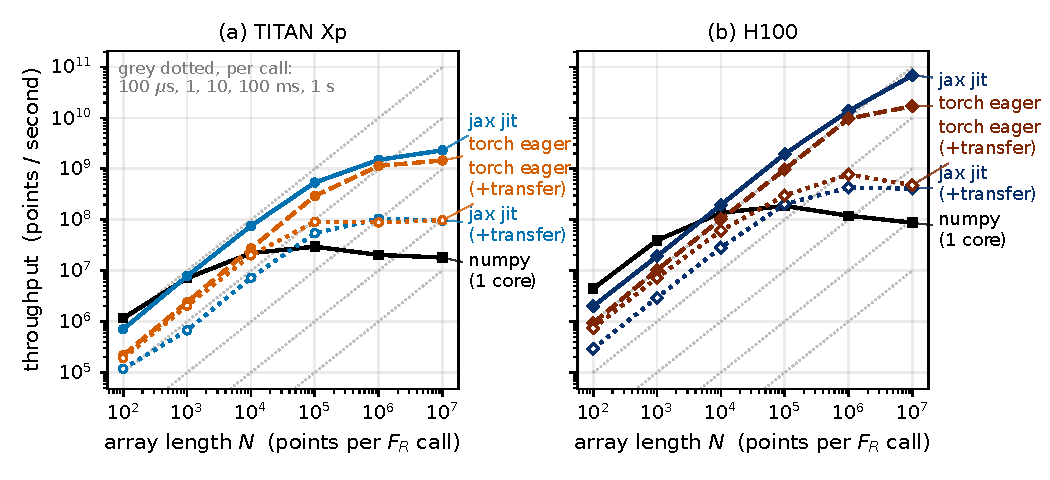
\includegraphics[width=0.48\textwidth,clip=]{../figures/g2_throughput/g2_throughput.pdf}
  \caption{Throughput of the radial force of a Plummer potential as a
    function of the number of points per call. The left panel shows the
    development machine, with \numpy\ on the CPU and \jax\ and \torch\
    on an NVIDIA TITAN~Xp; the right panel shows a node of the Trillium
    cluster, with an NVIDIA H100. Solid lines are compute-only, dashed
    lines include the transfer of inputs and outputs between host and
    device. Dotted lines mark constant wall time per call, which the GPU
    curves follow while launch-bound.}\label{fig:throughput}
\end{figure}

\section{Potentials}\label{sec:potential}

The \pot\ classes are the foundation of \galpy\ and were the first part
of the code that we migrated. The approach is the one of
\sectionname~\ref{sec:design-agnostic}: every private compute method
(\texttt{\_evaluate}, \texttt{\_Rforce}, \texttt{\_zforce},
\texttt{\_phitorque}, \texttt{\_dens}, \texttt{\_surfdens}, and the six
second derivatives) resolves the array namespace from its coordinates
and uses it throughout, and the public methods, through the coercion
decorator, bring scalar and \numpy\ inputs onto the namespace of any
backend input. For the majority of \galpy's potentials this was the
whole change, because they are elementary functions of the coordinates.
The remainder use special functions or tabulated quantities: the
basis-function and multipole expansions (\texttt{SCFPotential},
\texttt{MultipoleExpansionPotential}, and their disk variants) use the
associated Legendre and Gegenbauer polynomials; the power-law potential
with an exponential cutoff and the Einasto profile use incomplete gamma
functions; the double-exponential disk uses Bessel functions in a
Hankel-type integral; and the interpolated potentials and the King
profile evaluate splines. These go through the special-function router
and the interpolation layer of \sectionname~\ref{sec:design-numerics}.
All of the potentials, forces, and wrappers in \texttt{galpy.potential}
run on both backends, with the exception of the potentials that read
$N$-body snapshots through \texttt{pynbody} \citep{Pontzen2013} and
the interface \citep{Webb2020} to \texttt{AMUSE}
\citep{PortegiesZwart2009,Pelupessy2013,PortegiesZwart2018}, which
have no backend code. Even the adiabatic-contraction wrapper, whose
construction is a root find for the contracted profile, builds that
profile on the backend when one of its parameters, or a parameter of
one of the potentials that it contracts, is being differentiated. The
convenience functions that act on potentials (the circular velocity
and epicycle frequencies, the radius of a circular orbit of given
angular momentum or energy, the enclosed mass, and the tidal radius
and tidal tensor of \citealt{Webb2019}) are backend-aware as well;
those that require a root are solved with the shared root finder and
those that require an integral use Gauss--Legendre quadrature.

The derivatives of a potential with respect to the coordinates are, of
course, its forces and second derivatives, which \galpy\ implements by
hand. Under a backend, these can also be obtained by differentiating
the potential, and the agreement between the two is a strong test of
both:
for the basis-function expansions, the spiral arms, a rotating bar, and
composite potentials, the force by automatic differentiation agrees
with the hand-coded force
to a few parts in $10^{15}$, within twenty units in the last place
(\figurename~\ref{fig:adforces}), that is, the derivative that
automatic differentiation
produces is the analytic force up to rounding. While the test suite
checks these identities for every potential, under both backends and in
both modes, the derivatives that matter to the user are those with
respect to the parameters: a potential constructed with a backend array
as a parameter is differentiable with respect to that parameter through
every method. For example, the derivative of the radial force of a Miyamoto--Nagai 
potential with respect to its scale length $a$ reads with \jax\ as
\begin{code}
from galpy.potential import MiyamotoNagaiPotential
def Rforce_of_a(a):
    mp= MiyamotoNagaiPotential(amp=1.,a=a,b=0.3)
    return mp.Rforce(1.2,0.1)
dFR_da= jax.grad(Rforce_of_a)(0.5)
\end{code}
and the same with \torch\ is
\begin{code}
a= torch.tensor(0.5,requires_grad=True)
mp= MiyamotoNagaiPotential(amp=1.,a=a,b=0.3)
mp.Rforce(torch.tensor(1.2),
          torch.tensor(0.1)).backward()
a.grad # dFR/da
\end{code}
All 47 potentials that can be constructed from parameters alone are
differentiable with respect to their amplitude (or, for the King
model, its mass) in this way, both eagerly and under
compilation. \figurename~\ref{fig:paramgrad}
displays the accuracy of these parameter derivatives and a small
example of their use, the recovery of the scale length of a Plummer
potential from its force by gradient descent. The parameters of a
potential constructed from a density, as the basis-function and
multipole expansions and their disk variants can be, carry the
derivative through the expansion coefficients.

\begin{figure*}[t!]
  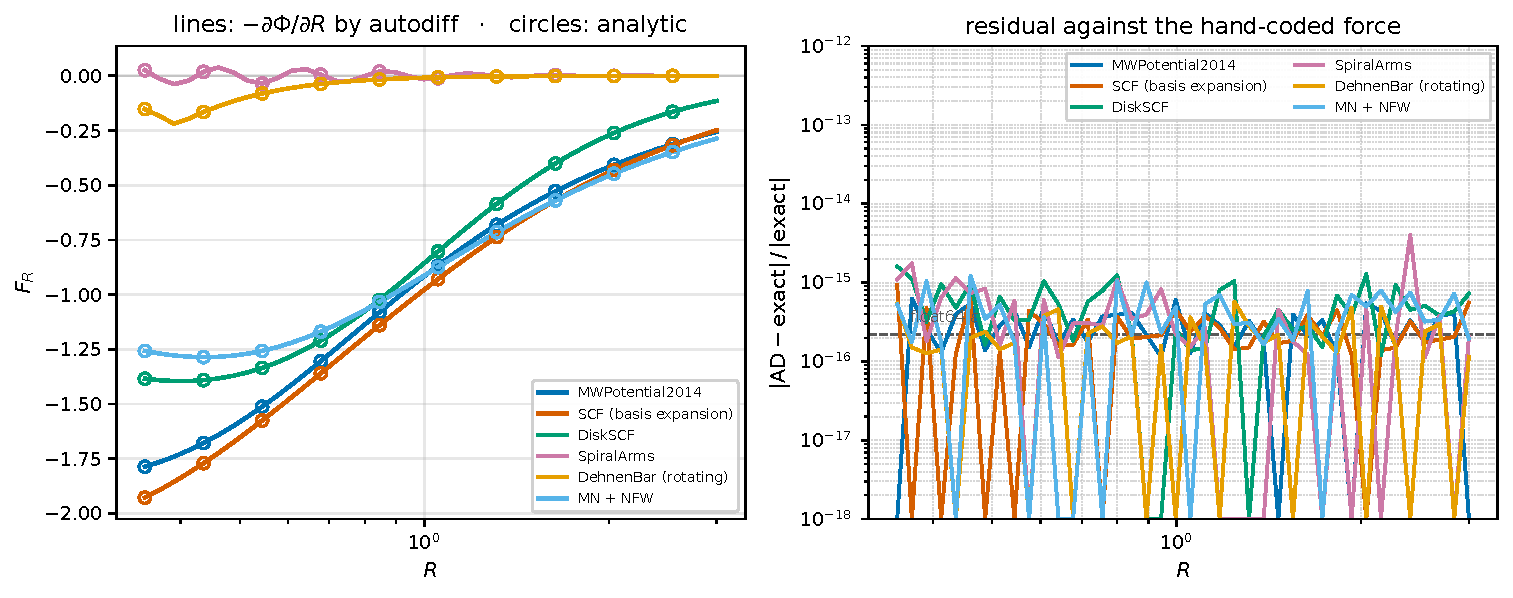
\includegraphics[width=\textwidth,clip=]{../figures/gF1_autodiff_forces/gF1_autodiff_forces.pdf}
  \caption{The radial force by automatic differentiation of the
    potential compared with the hand-coded force, for the Milky-Way
    model, a basis-function expansion and its disk variant, spiral arms,
    a rotating bar, and a disk-plus-halo composite. Left: the force along
    $R$ in the mid-plane, lines from automatic differentiation and
    circles from the analytic implementation. Right: the relative
    difference between the two, which is at the level of the
    double-precision rounding error.}\label{fig:adforces}
\end{figure*}

\begin{figure*}[t!]
  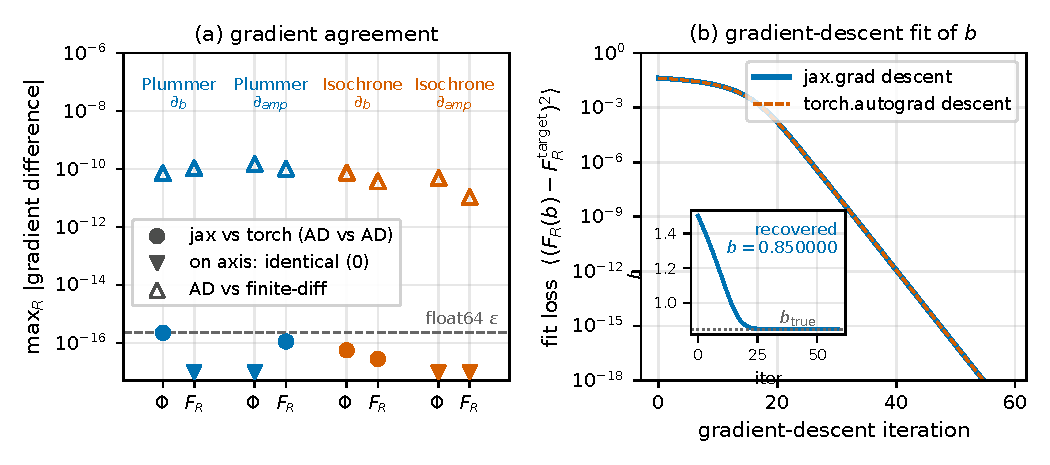
\includegraphics[width=\textwidth,clip=]{../figures/g3_param_gradients/g3_param_gradients.pdf}
  \caption{Derivatives of potentials with respect to their parameters.
    The left panel shows, for the Plummer and isochrone potentials, the
    largest difference between the derivatives of the potential and of
    the radial force with respect to the amplitude and scale parameters
    computed with \jax\ and with \torch\ (circles, at the level of the
    double-precision rounding error; where the two are bit-identical, the
    difference is zero and cannot be shown on the logarithmic axis, which
    the filled triangles on the axis mark) and between either of these and a
    central finite difference (open triangles, at the level of the
    finite-difference error). The right panel displays the recovery of
    the scale length of a Plummer potential from the radial force at a
    set of points by gradient descent on the derivative, starting from
    $b=1.5$ and converging to the true $b=0.85$, with both
    backends.}\label{fig:paramgrad}
\end{figure*}

The backend potentials differ from the \numpy\ ones in a few respects.
Where \galpy\ computes an integral over a potential adaptively on the
\numpy\ path, as for the enclosed mass of a general density or the
surface density, the backend computes a fixed-order Gauss--Legendre
approximation; we set the order such that the two agree, but the backend
result is an approximation of fixed cost rather than an adaptive one. Interpolated potentials evaluate
the same spline as \scipy\ does, to within one unit in the last place,
by converting the fitted spline to a piecewise-polynomial table; they are
differentiable in the evaluation point and, when they are built from a
potential or function with a parameter that is being differentiated,
also in the tabulated values, because the table and the spline
coefficients are then computed on the backend and the derivative with
respect to the parameter passes through them.
A potential that moves along a precomputed orbit, as the
\texttt{MovingObjectPotential}, interpolates that orbit on the backend
when the orbit was integrated there, such that the field of the moving
object is differentiable with respect to everything that the orbit
depends on, and lives on the GPU when the orbit does; an orbit
integrated with \numpy\ stays on \numpy\ and the field is computed at
backend coordinates. And a \python\ branch on the
value of a stored parameter, such as the special case of a vanishing
scale length, is harmless when the parameter is differentiated eagerly
but fails when the parameter is traced inside a compiled ODE solve; we
replaced such branches where we found them, but authors of new
potentials should keep this behavior in mind.

New potentials are written as before: a class that inherits from
\pot\ and implements \texttt{\_evaluate}, \texttt{\_Rforce}, and
\texttt{\_zforce}. If these are written with the resolved namespace
rather than with \numpy\ directly, as illustrated in \figurename~\ref{fig:newpot},
the new potential runs on every backend and can be differentiated with
respect to its parameters without any further work, and the test suite's
automatic checks of new potentials are run under every backend. A test
checks that no migrated potential calls \numpy\ directly in a compute
method.

\begin{figure}[t!]
\begin{codefig}
from galpy.potential import Potential
from galpy.backend import get_namespace
class MNLikePotential(Potential):
    # a Miyamoto-Nagai disk written for every backend
    def __init__(self,amp=1.,a=1.,b=0.1,
                 normalize=False):
        Potential.__init__(self,amp=amp)
        self._a= a
        self._b2= b**2
        if normalize: self.normalize(normalize)
    def _evaluate(self,R,z,phi=0.,t=0.):
        xp= get_namespace(R,z)
        s= self._a+xp.sqrt(z**2+self._b2)
        return -1./xp.sqrt(R**2+s**2)
    def _Rforce(self,R,z,phi=0.,t=0.):
        xp= get_namespace(R,z)
        s= self._a+xp.sqrt(z**2+self._b2)
        return -R*(R**2+s**2)**-1.5
    def _zforce(self,R,z,phi=0.,t=0.):
        xp= get_namespace(R,z)
        sqb= xp.sqrt(z**2+self._b2)
        s= self._a+sqb
        return -z*s/sqb*(R**2+s**2)**-1.5
# differentiate an orbit in it w.r.t. the scale length a
def final_z(a):
    o= Orbit(jnp.asarray([1.,0.1,1.1,0.1,0.05,0.]))
    mp= MNLikePotential(a=a,b=0.3,normalize=1.)
    o.integrate(ts,mp,method='diffrax')
    return o.z(ts[-1])
jax.grad(final_z)(0.5)
\end{codefig}
\caption{A new \pot\ class written for every backend. The only
  difference from a class written for \numpy\ is that the array
  functions are taken from the namespace resolved from the coordinates
  (\texttt{xp}) rather than from \numpy. The class can then be used, and
  differentiated, like any other potential; the last lines take the
  derivative of the final height of an orbit with respect to the scale
  length of the new potential.}\label{fig:newpot}
\end{figure}

\section{Orbit integration}\label{sec:orbit}

\subsection{Three ways to integrate an orbit}\label{sec:orbit-paths}

\orb\ instances are set up and integrated as before, but an \orb\ instance whose
initial condition is a backend array, or whose potential carries a
backend parameter, is integrated in one of two new ways, depending on
what is to be differentiated. The first integrates the equations of
motion inside the backend, with the backend's own ODE solver:
\diffrax\ \citep{Kidger2021} for \jax, with an eighth-order
Dormand--Prince method, and \texttt{torchdiffeq} \citep{Chen2018} or
\torchode\ \citep{LienenGunnemann2022} for \torch, with a fifth-order method.
The equations of motion are those of \galpy's \cc\ integrators,
evaluated in rectangular coordinates through the backend force layer,
and the default tolerances are $10^{-12}$. Because the whole integration
is then a backend program, everything that enters it can be
differentiated: the initial condition, the potential's parameters, the
integration times. $N$ orbits are integrated in a single solve along a
batch axis, with per-orbit time grids if desired, and the solve runs on
a GPU when the initial conditions do. This is the path to use for
derivatives with respect to the parameters of the potential, 
as in the following example:
\begin{code}
def final_R(b):
    o= Orbit(jnp.asarray(ic))
    pp= PlummerPotential(amp=1.,b=b)
    o.integrate(ts,pp,method='diffrax')
    return o.R(ts[-1])
dR_db= jax.grad(final_R)(0.6)
\end{code}
and under \torch:
\begin{code}
b= torch.tensor(0.6,requires_grad=True)
o= Orbit(torch.as_tensor(ic))
pp= PlummerPotential(amp=1.,b=b)
o.integrate(torch.as_tensor(ts),pp,method='torchode')
o.R(ts[-1]).backward() # b.grad = dR/db
\end{code}
Second derivatives are available under \jax\ by selecting the direct
adjoint through the \texttt{inbackend\_kwargs} keyword, and
\texttt{jax.vmap} over initial conditions works, with one caveat
discussed below. \figurename~\ref{fig:orbitsens} displays the simplest
use of these derivatives: the sensitivity of an orbit to its initial
conditions as a function of time, which the solver's derivative gives
for free and which finite differences confirm, and a Gauss--Newton fit
of the launch velocity of an orbit to a target end point using the
Jacobian of the integration, which converges quadratically to machine
    precision in a handful of iterations.

\begin{figure*}[t!]
  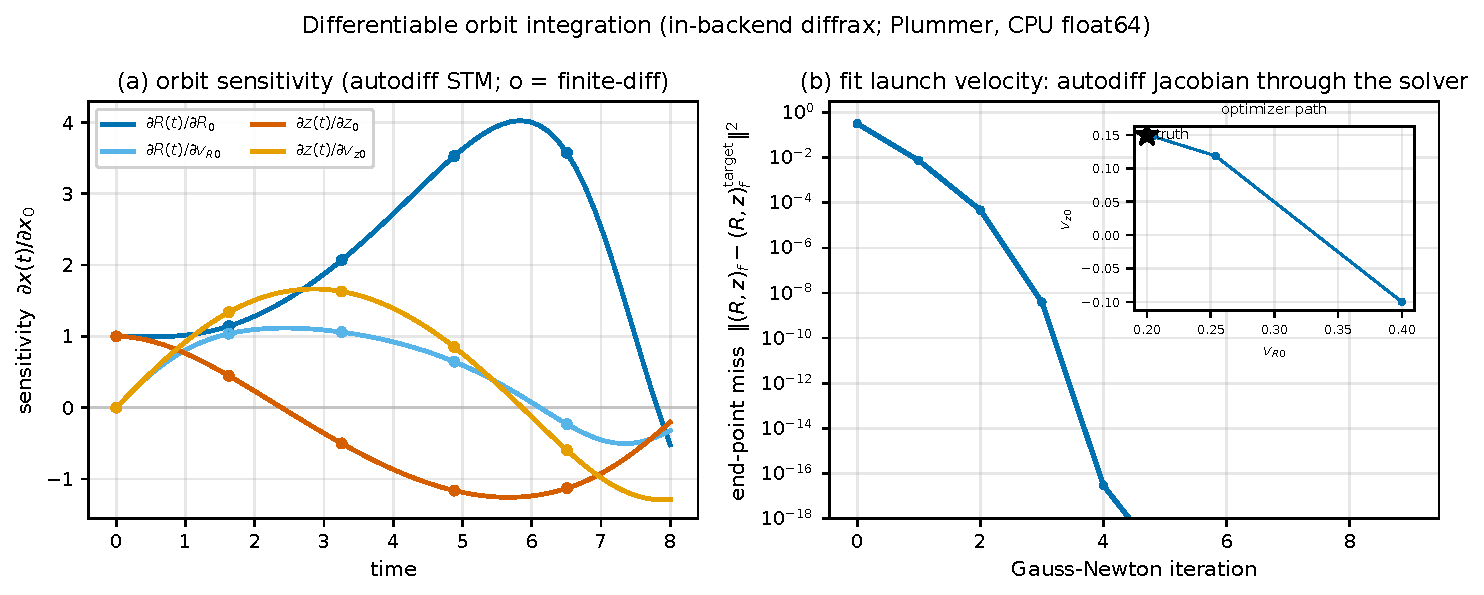
\includegraphics[width=\textwidth,clip=]{../figures/g7_orbit_sensitivity/g7_orbit_sensitivity.pdf}
  \caption{Derivatives of an in-backend orbit integration. Left: the
    sensitivities $\partial R(t)/\partial R_0$, $\partial R(t)/\partial v_{R,0}$,
    $\partial z(t)/\partial z_0$, and $\partial z(t)/\partial v_{z,0}$ of an
    orbit in a Plummer potential by reverse-mode differentiation through
    the \diffrax\ solve (lines) and by central finite differences
    (circles). Right: the squared distance between the end point of the
    orbit and a target as the launch velocity $(v_{R,0},v_{z,0})$ is
    fit by Gauss--Newton iterations on the Jacobian of the integration;
    the inset shows the path of the fit. The derivative through the
    solver agrees with the finite differences, and the fit that uses it
    converges in a handful of iterations.}\label{fig:orbitsens}
\end{figure*}

The second way uses \galpy's compiled \cc\ integrators, which are much
faster than a solver that runs inside \jax\ or \torch\ on a CPU (for a
single orbit in the Milky-Way model \texttt{MWPotential2014}, 
about ten times faster than the
\diffrax\ solve and a hundred times faster than \texttt{torchdiffeq}),
but which are opaque to automatic differentiation. What they can provide is the derivative of the
orbit with respect to its initial condition, through the variational
equations that \galpy\ integrates alongside the orbit in \cc\
(\appendixname~\ref{app:dxdv}). When a \galpy\ orbit with a backend
initial condition is integrated with a \cc\ method, the \cc\ integrator
returns both the orbit and the state-transition matrix
$\vec{M}(t) = \partial \vecw(t)/\partial \vecw(0)$, and a custom
derivative rule tells the backend that the derivative of the orbit with
respect to the initial condition is $\vec{M}$; the reverse-mode
derivative of any function of the orbit is then a single product of
$\vec{M}^T$ with the cotangent, without a second call to \cc. For a
six-dimensional orbit and a Runge--Kutta method, the six columns of
$\vec{M}$ are integrated together with the orbit as a 42-component
state; for the symplectic methods, the deviation vectors are propagated
through the same drift and kick steps as the orbit. The derivative is
exact to the precision of the solver: \figurename~\ref{fig:icjacobian}
compares the state-transition matrix of a Milky-Way orbit over 3\,Gyr
from the \cc\ variational equations with reverse-mode automatic
differentiation through
\diffrax\ and through \texttt{torchdiffeq} and with finite differences
of independently integrated orbits, and the four agree to a few parts in
$10^{10}$. In code, nothing marks the difference between the two paths except the
method:
\begin{code}
def end_point(ic):
    o= Orbit(ic)
    o.integrate(ts,MWPotential2014,
                method='dop853_c') # C + variational
    return jnp.stack([o.R(ts[-1]),o.z(ts[-1])])
M= jax.jacrev(end_point)(jnp.asarray(ic)) # STM rows
\end{code}
and a batch of orbits is differentiated with \texttt{jax.vmap},
\begin{code}
Ms= jax.vmap(jax.jacrev(end_point))(ics) # ics: (N,6)
\end{code}
This path gives derivatives with respect to the initial
conditions only, and to first order only; the variational equations do
not carry derivatives with respect to the parameters of the potential,
which must come from the in-backend solve.

\begin{figure*}[t!]
  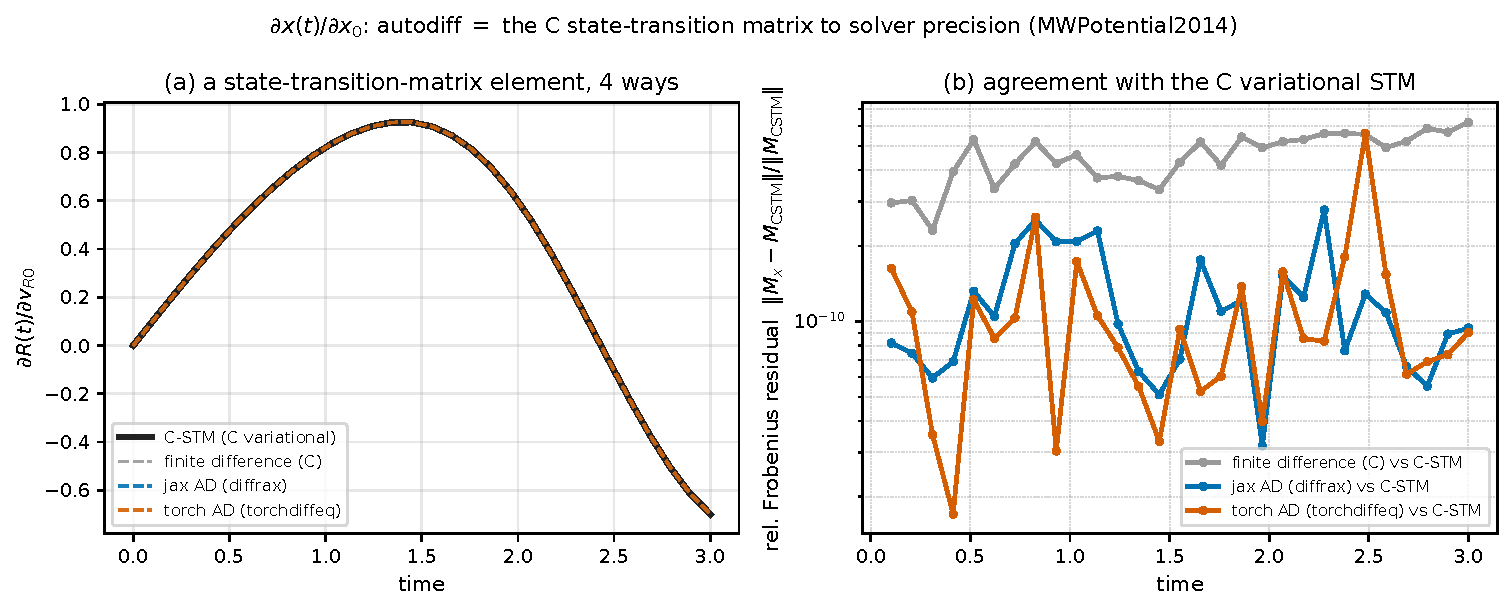
\includegraphics[width=\textwidth,clip=]{../figures/g16_icjacobian_precision/g16_icjacobian_precision.pdf}
  \caption{The derivative of an orbit with respect to its initial
    condition, in four ways. For a Sun-like orbit in \texttt{MWPotential2014}
    integrated for 3\,Gyr, the left panel shows one element of the
    state-transition matrix, $\partial R(t)/\partial v_{R,0}$, from the
    \cc\ variational equations, from a finite difference of the \cc\
    orbit, and from reverse-mode automatic differentiation through the
    \diffrax\ and \texttt{torchdiffeq} solvers. The right panel shows the
    relative Frobenius norm of the difference between each of the
    latter three and the variational result; all agree to a few parts in
    $10^{10}$.}\label{fig:icjacobian}
\end{figure*}

\galpy\ chooses between the two automatically. An \orb\ whose
initial condition is being differentiated---a traced \jax\ array or a
\torch\ tensor that requires a gradient---and that is integrated with
a \cc\ method, in a potential that has \cc\ second derivatives, with
non-traced times and non-traced potential parameters, uses the \cc\
integrator and its variational equations. In every other case in
which something is differentiated, in particular whenever a potential
parameter is traced or when the integration is to run on a GPU, the
in-backend solver is used, under the name \texttt{method='diffrax'},
\texttt{'torchode'}, or \texttt{'torchdiffeq'}, which can also be
requested directly. When nothing is being differentiated, that is, for
a concrete backend initial condition, a \cc\ method integrates in
\cc\ as before, without the variational equations, and only its result
is a backend array; this is not a third way of integrating but the old
one, and it means that a backend initial condition costs nothing until
it is differentiated. The pure-\python\ integrators of \galpy\
(\texttt{method='odeint'}, the \python\ leapfrog, and so on) are not
routed at all: given a backend initial condition they integrate in
\numpy\ and return a backend array that is not differentiable, with a
warning.

After integration, the orbit's methods work as before on backend
arrays: positions and velocities at the integration times or, by
interpolation with an in-backend spline, between them; energies and
angular momenta; peri- and apocenter radii and maximum height, both
from the integrated orbit and analytically through the action--angle
code of \sectionname~\ref{sec:aa} \citep{MackerethBovy2018}; and the transformations to observed
coordinates. Initializing an orbit from observed coordinates with
backend arrays works as well, such that a derivative with respect to a
star's distance or proper motion is available.

\subsection{Backend symplectic integrators for many orbits}\label{sec:orbit-leapfrog}

The in-backend solvers of \sectionname~\ref{sec:orbit-paths} are
adaptive Runge--Kutta methods: accurate, but expensive, because a step
of \diffrax's eighth-order Dormand--Prince method evaluates the force
thirteen times, and, as discussed in
\sectionname~\ref{sec:orbit-limitations}, their adaptive steps
complicate the derivative of a batch of orbits. For large batches of
orbits in a smooth potential, where modest precision suffices and the
cost is dominated by the force evaluations, a symplectic integrator
with a fixed step is the better tool: it evaluates the force once per
step, its energy error oscillates without a secular drift, it keeps
little state per orbit, and its fixed steps make the derivative of a
batch straightforward. \galpy\ therefore also integrates inside the
backends with a kick-drift-kick leapfrog with a constant step,
\texttt{method='leapfrog\_jax'} and \texttt{method='leapfrog\_torch'},
as for example in the following:
\begin{code}
o= Orbit(jnp.asarray(ics)) # ics: (N,6)
o.integrate(ts,MWPotential2014,method='leapfrog_jax',
            inbackend_kwargs={'nsteps':8000})
\end{code}
The same route provides backend versions of the fourth- and
sixth-order symplectic integrators \citep{Yoshida1990,Kinoshita1991}
of \galpy's \cc\ library, \texttt{method='symplec4\_jax'} and
\texttt{'symplec6\_jax'} (and their \torch\ twins), which evaluate the
force three and seven times per step and agree with their \cc\
counterparts at the same step to rounding; they are the better choice
when more than a few digits are wanted: for the batch of disc orbits of
\sectionname~\ref{sec:orbit-speed}, 450 sixth-order steps over 2\,Gyr
(3150 force evaluations) reach the worst-case accuracy of the adaptive
Dormand--Prince solve at tolerances of $10^{-8}$, which takes about 250
steps (3250 force evaluations).
The leapfrog is second order: its error falls by a factor of four per
halving of the step, and in a static potential its energy error
oscillates without the secular drift that a non-symplectic
second-order method with the same steps shows; we verified both for a
batch of 2000 orbits in \texttt{MWPotential2014} with a moving
satellite and the acceleration of a non-inertial frame, against the
\cc\ integrator. For reverse-mode
derivatives, the steps are grouped into blocks under the backend's
checkpointing (\texttt{jax.checkpoint} or \texttt{torch.utils.checkpoint}),
such that the derivative stores the state at the start of each block and
the states within one block, about $2\sqrt{N_\mathrm{steps}}$ states
rather than $N_\mathrm{steps}$: for $10^5$ orbits and 8000 steps in
\texttt{MWPotential2014}, the compiled \jax\ derivative needs 1.4\,GB of
temporary memory instead of 39\,GB. The derivatives agree with
Richardson-extrapolated central differences of the same integration to
$10^{-10}$, and the \jax\ and \torch\ versions agree with each other to
$2\times10^{-14}$. An initial condition in single precision is
integrated in single precision throughout, including the times and the
forces, which matters on GPUs with a low double-precision rate
(\sectionname~\ref{sec:orbit-speed}). Forces that do not derive from a
potential, such as dynamical friction or the Coriolis force of a
rotating frame, which \galpy\ marks with the \texttt{isConservative}
attribute, raise an error, because the closing kick would evaluate
them at the half-step velocity and the method would then converge only
at first order. As a second-order method, the leapfrog needs small steps
to be precise: for $10^4$ disc orbits integrated for 0.36\,Gyr, 1000
leapfrog steps (1000 force evaluations) give a worst-case position
error of $3\times10^{-4}$ (in units of $R_0$), while 250 Dormand--Prince
steps (3250 force evaluations) give $4\times10^{-7}$. The leapfrog is
therefore the method of choice when the force is expensive to evaluate
and modest precision suffices, the sixth-order integrator when the
orbits share a timescale and precision matters, and the adaptive
Runge--Kutta solvers remain the choice for batches that mix
timescales.

\subsection{Variational equations and chaos}\label{sec:orbit-dxdv}

The variational equations that the \cc\ state-transition matrix relies
on were part of \galpy\ for planar orbits since 2011; as part of this
work, we extended them to three-dimensional orbits, to all of the \cc\
integrators including the symplectic ones, to one-dimensional orbits,
and to dissipative, velocity-dependent forces, and we released them in
\galpy\ \flag{v1.12}. \appendixname~\ref{app:dxdv} gives the equations
and the checks that we applied to them. Their user-facing form is
\texttt{Orbit.integrate\_dxdv}, which integrates an orbit together with a
deviation vector or with the full state-transition matrix, and
\texttt{Orbit.lyapunov}, which computes the largest Lyapunov exponent, or
the spectrum, by the renormalization method of \citet{Benettin1980a,Benettin1980b},
for example as
\begin{code}
o= Orbit([0.8,0.3,0.75,0.,0.2,0.])
o.integrate_dxdv([1.,0.,0.,0.,0.,0.],ts,
                 MWPotential2014,method='dop853_c')
o.getOrbit_dxdv() # the deviation along the orbit
o.lyapunov(ts,MWPotential2014,method='dop853_c',
           renorm_every=10)
\end{code}
For
example, for the H\'enon--Heiles potential at $E=1/8$, the exponent of a chaotic orbit
converges into the range quoted in the literature while that of a
regular orbit at the same energy decays as $\ln t/t$
(\figurename~\ref{fig:lyapunov}). Like the variational equations
themselves, these are \numpy\ and \cc\ features that do not require
the backends: they accept backend initial conditions, but run on the
CPU, return \numpy\ arrays, and are not differentiable.

\begin{figure*}[t!]
  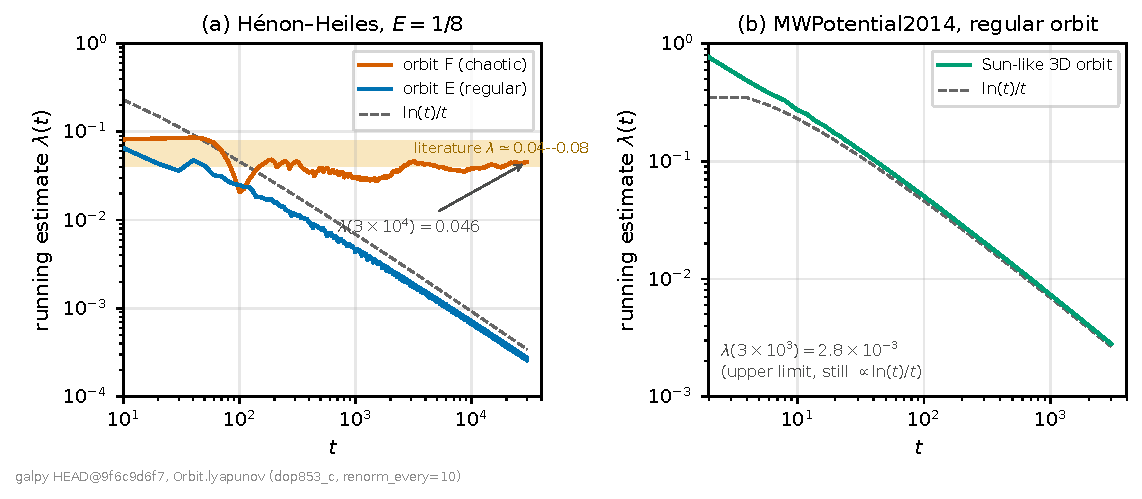
\includegraphics[width=\textwidth,clip=]{../figures/g10_lyapunov/g10_lyapunov.pdf}
  \caption{Largest Lyapunov exponent from \texttt{Orbit.lyapunov}, as a
    running estimate against time. Left: a chaotic and a regular orbit
    in the H\'enon--Heiles potential at $E=1/8$; the shaded band is the
    range of values in the literature for the chaotic orbit, and the
    dashed line is the $\ln t/t$ decay expected for a regular orbit.
    Right: a Sun-like orbit in \texttt{MWPotential2014}, which is
    regular. The estimate for the chaotic  H\'enon--Heiles orbit converges into the range
    found in the literature, while that for the regular orbit decays as
    expected.}\label{fig:lyapunov}
\end{figure*}

\subsection{Limitations}\label{sec:orbit-limitations}

In-backend orbit integration has a few limitations. 
By default, the derivative of an in-backend solve with respect to its
inputs differentiates through the solver's adaptive steps, which is
correct for a single orbit; when a batch of orbits is differentiated
under \texttt{jax.vmap}, however, the adaptive steps of one orbit depend
on the others and the derivative is wrong by several percent.
The remedy is to integrate with a fixed number of steps when
differentiating a batch, which \galpy\ does where it integrates batches
internally and which the user should do as well; \galpy\ warns when a
batch of orbits is differentiated through an adaptive in-backend
solve under \jax, where it can detect the derivative being taken, and
points at the fixed-step option. \texttt{torchdiffeq}
has no batching rule, such that a batch of orbits under \torch\ is a
\python\ loop unless \torchode\ is used. The eighth-order method of
\texttt{torchdiffeq} carries a gradient error of about $10^{-5}$ in its
backward pass, which is why \galpy\ uses its fifth-order method. Additionally, the
pure-\python\ integrators implemented in \galpy\ are not routed to the
backends (\sectionname~\ref{sec:orbit-paths}); they can run on a
backend under the forced mode of \sectionname~\ref{sec:design-choosing},
but are slow there, because each step is a separate set of array
operations, and we do not recommend it.
Finally, the \cc\ integrators cannot be used on a GPU at
all; their derivative rule runs the integration on the CPU.

\subsection{Speed}\label{sec:orbit-speed}

\figurename~\ref{fig:orbitspeed} compares the wall time of integrating
$N$ orbits for 2\,Gyr in \texttt{MWPotential2014} with the \cc\ integrator,
which parallelizes over orbits with OpenMP, on one core and on the 36
physical cores of the CPU node used in this work, and with the in-backend solvers on one CPU
core and on two GPUs. The absolute times depend on the specifics of the
problem, so we focus on the relative trends. On a single CPU core, the compiled \jax\
solve and the eager \torch\ solve cost about the same per orbit as the
\cc\ path for large batches, but they start from a floor of one to a
few seconds, set by compilation and kernel launches, that the \cc\ path
does not have, such that the \cc\ path is faster for up to a few
thousand orbits; the compiled solve additionally takes seconds to
compile, a cost that is paid once per shape of the problem. The \cc\
path is also the only one that makes use of more cores: its OpenMP loop
speeds up almost linearly to the 36 cores of our node for $10^4$ orbits
or more, eager \torch\ gains at most a factor of 3.5 (on 16 threads),
and compiled \jax, whose runtime keeps no more than a few cores busy,
gains nothing. The GPUs amortize a floor of half a second to a second
over the batch: the compiled \jax\ lines overtake one-core \cc\ at a
few hundred orbits and the \torch\ lines at a few thousand. The
consumer GPU, which executes double-precision arithmetic at one
thirty-second of its single-precision rate, never beats the 36-thread
\cc\ node with the adaptive solvers, while the H100 passes it at about
$10^4$ orbits and is 5 to 9 times cheaper per orbit for
$N\geq3\times10^5$. The
sixth-order symplectic integrator of
\sectionname~\ref{sec:orbit-leapfrog}, with the common step of that
section, is the cheapest in-backend route for this batch of disc
orbits, because its state per orbit is a fraction of the adaptive
solvers' and its steps are the same for every orbit: on one CPU core
it costs half of the adaptive \cc\ path, on the consumer GPU it beats
the 36-thread \cc\ node for $N\geq10^4$, which the adaptive solvers
cannot there, and on the H100 it is 3 to 7 times cheaper than the
adaptive solve on the same card and about 30 times cheaper than the
36-thread \cc\ node for $N\geq10^5$; for fewer
orbits, its compiled step loop is bound by its kernel launches, at
0.3--0.4\,s for the 450 steps on either GPU. The derivative of an orbit with respect to its
initial condition follows the same pattern
(\figurename~\ref{fig:icderivcost}): the \cc\ variational integrator
computes it fastest for a single orbit, by one to three orders of
magnitude over the backend solvers, and the GPU overtakes it at
batches of a few hundred orbits.

To gauge what GPU-native code could add, we also compiled \galpy's
\cc\ implementations of \texttt{MWPotential2014} and of its integrators
as a CUDA kernel that integrates one orbit per GPU thread; this is an
experiment and not part of \galpy. After restructuring the kernel, such
that the force is evaluated by a single out-of-line function and
threads pick up a new orbit when theirs is done, \texttt{dop853} on the
H100 is 4 to 11 times faster per orbit than \galpy's compiled \jax\
integrator on the same GPU and 30 to 90 times faster than the \cc\
integrator on the 36 cores of our CPU node (2.4\,$\mu$s per orbit
with a direct port of \galpy's \cc\ code and 0.9\,$\mu$s with special
functions rewritten for the GPU), while agreeing with the latter to
within its truncation error (\figurename~\ref{fig:orbitspeed}). The
kernel is limited by per-thread state: an adaptive eighth-order step
keeps $\approx$880\,B per orbit live, so few threads fit on each
multiprocessor. \galpy's sixth-order symplectic integrator with one
common step for the whole batch reaches the same accuracy with 15\%
fewer force evaluations and a fraction of the state, and runs another
3 to 4 times faster. These numbers hold for a smooth, cheap potential
and near-solar disc orbits with similar dynamical times, for which one
step suits every orbit; a batch that mixes very different timescales,
or has close encounters or a rapidly varying potential, has to step at
the rate of its fastest orbit, and there adaptive integration wins.
Such kernels are not differentiable, so they would complement the
backend integrators rather than replace them
(\sectionname~\ref{sec:conclusion}).

\galpy\ is not the only galactic-dynamics code that integrates orbits
with \diffrax: \texttt{galax} \citep{Starkman2026}, a re-implementation
of \texttt{gala} in \jax, does so by design, and comparing the two
checks that the cost of the in-backend solve is in the solver and the
potential rather than in the library around them. The green lines in
\figurename~\ref{fig:orbitspeed} show this comparison for the same
orbits, potential, and tolerances. When we make \texttt{galax} control
its step size per orbit, as \galpy\ does, the two codes take the same
time to within 13 per cent on both GPUs for batches of $10^5$ orbits or
more; for smaller batches, whose cost is dominated by fixed overheads,
they differ by up to a factor of 1.6, in opposite directions on the two
GPUs. In its default mode, \texttt{galax} integrates the whole batch as
one system with a single step-size controller, whose error estimate is
the root-mean-square over all orbits, such that one sequence of steps
serves every orbit; this is cheaper per orbit for large batches, by a
factor of two to three, at the price of an error control that holds
only in the batch-averaged sense and that depends on which orbits
happen to be in the batch. \galpy\ keeps the per-orbit control.

\begin{figure*}[t!]
  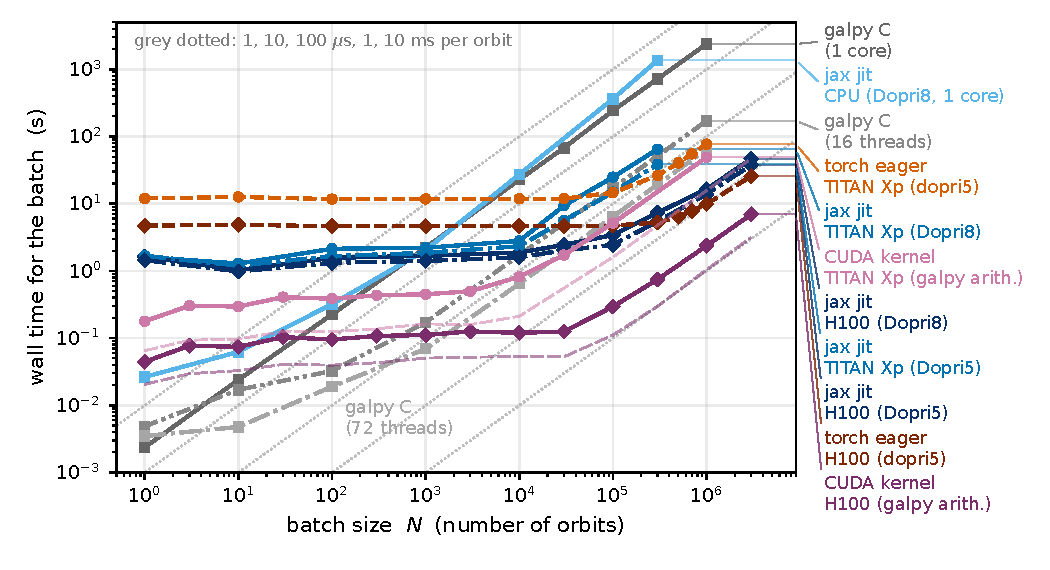
\includegraphics[width=\textwidth,clip=]{../figures/g12_inbackend_orbit_gpu/g12_inbackend_orbit_gpu.pdf}
  \caption{Wall time for integrating $N$ orbits for 2\,Gyr in
    \texttt{MWPotential2014} with relative and absolute tolerances of
    $10^{-8}$, on (a) the CPU, (b) the TITAN~Xp, and (c) the H100; each
    label repeats the style of its line. Grey: \galpy's \cc\ integrator
    \texttt{dop853\_c}, which parallelizes over orbits with OpenMP, on
    one core, 16 threads, and the 36 physical cores of the node; the
    latter is repeated in the GPU panels for reference. Blue: the
    in-backend \diffrax\ solve under \jax, compiled, with the
    eighth-order method that \galpy\ uses by default and with a
    fifth-order method that performs the same number of force
    evaluations as the \torch\ solve, and the in-backend sixth-order
    symplectic integrator (\texttt{symplec6\_jax}) with 450 common
    steps over the 2\,Gyr, the step at which its worst-case position
    error over the batch equals that of the adaptive solve. Orange and
    red: the eager \texttt{torchdiffeq}
    solve. Green: \texttt{galax} with its default batched step-size
    control and with per-orbit control as in \galpy. Purple: an
    experimental CUDA port of \galpy's \cc\ forces and \texttt{dop853}
    that integrates one orbit per GPU thread (not part of \galpy\ and
    not differentiable), with a direct port of \galpy's \cc\ code and
    with special functions rewritten for the GPU, including the copies
    between host and device, which keep these lines flat up to
    $N\approx10^4$. Light grey dotted lines mark a constant cost per
    orbit, and the arrows point towards lower wall time.}\label{fig:orbitspeed}
\end{figure*}

\begin{figure*}[t!]
  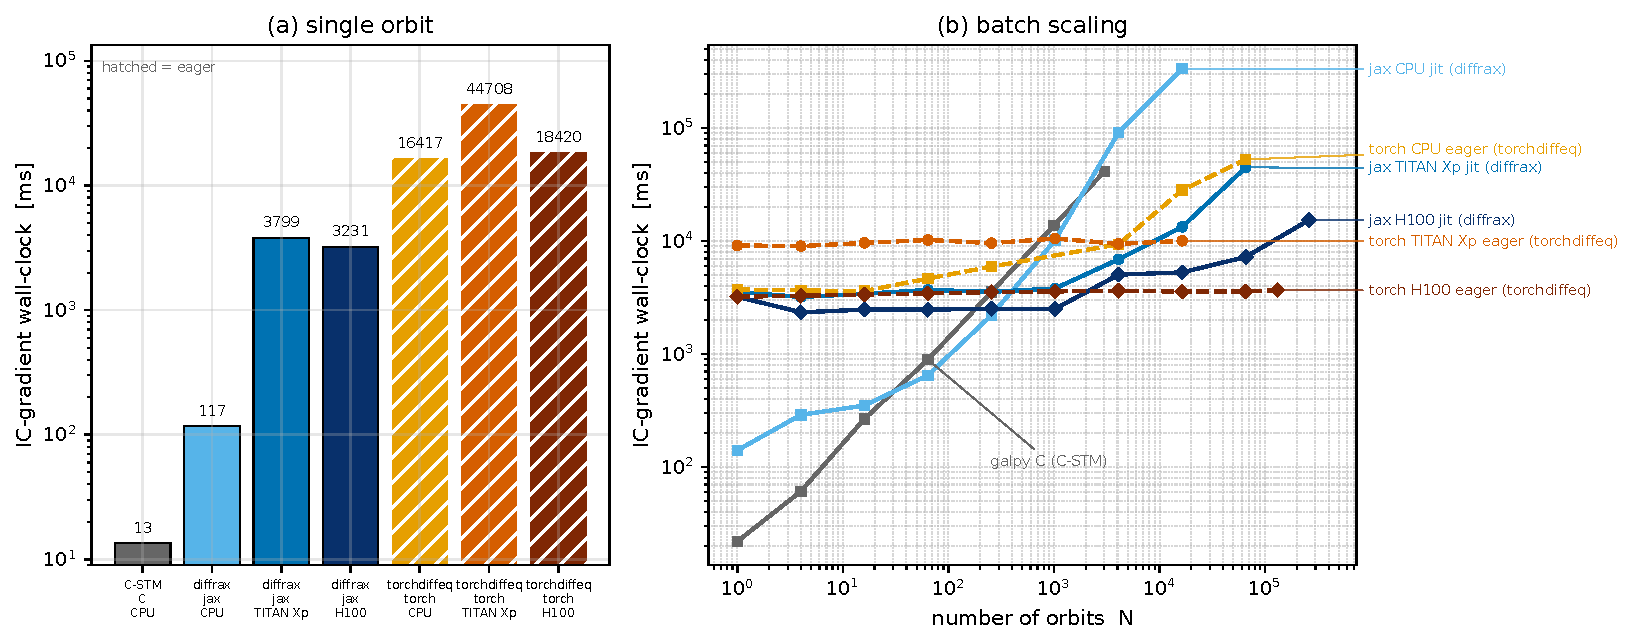
\includegraphics[width=\textwidth,clip=]{../figures/g15_icderiv_speed/g15_icderiv_speed.pdf}
  \caption{Cost of the derivative of an orbit with respect to its
    initial conditions, for a 2\,Gyr orbit in \texttt{MWPotential2014}.
    Left: wall time for a single orbit with the \cc\ variational
    integrator and by reverse-mode differentiation through the
    \diffrax\ and \texttt{torchdiffeq} solves on the CPU and the two
    GPUs; hatched bars are eager and solid bars compiled. Right: the same as a function of the
    number of orbits differentiated at once. The \cc\ variational
    integrator is the fastest way to obtain the derivative of a single
    orbit, while a GPU overtakes it for large batches. All CPU timings use
    one core.}\label{fig:icderivcost}
\end{figure*}


\section{Action--angle coordinates}\label{sec:aa}

\subsection{General approach}\label{sec:aa-general}

The action--angle module is where \galpy's numerical methods are
concentrated: root finding for the turning points of an orbit,
quadrature of the action integrals between them, and, for the
approximate methods, auxiliary orbit integrations. All of
\texttt{galpy.actionAngle} runs on the backends except for the interface
to the external torus-mapping code, which is excluded for good. The
public interface is unchanged: an \texttt{actionAngle} instance is set up
for a potential and called with phase-space positions, through
\texttt{\_\_call\_\_} for the actions, \texttt{actionsFreqs} for actions
and frequencies, and \texttt{actionsFreqsAngles} for all three; a call
with backend arrays, or with a potential that carries a backend
parameter, computes with that backend. Because these methods take a
variable number of positional arguments, they resolve the namespace and
promote scalars internally rather than through the coercion decorator
of the potentials. Derivatives are available with respect to the
phase-space position and, through the Python implementations, with
respect to the parameters of the potential; these parameter derivatives
agree with finite differences in which the potential and the
\texttt{actionAngle} instance are rebuilt from the perturbed parameter
to a few parts in $10^{10}$ for the St\"{a}ckel, adiabatic, and
spherical methods. \figurename~\ref{fig:aasens} shows the two kinds of
derivative for the isochrone potential, where the actions are known in
closed form: the derivatives of the radial and vertical actions with
respect to the radial velocity, and the derivative of the radial action
with respect to the scale radius of the potential, which is the
derivative that an inference loop uses when it adjusts the potential
to match measured actions.

\begin{figure*}[t!]
  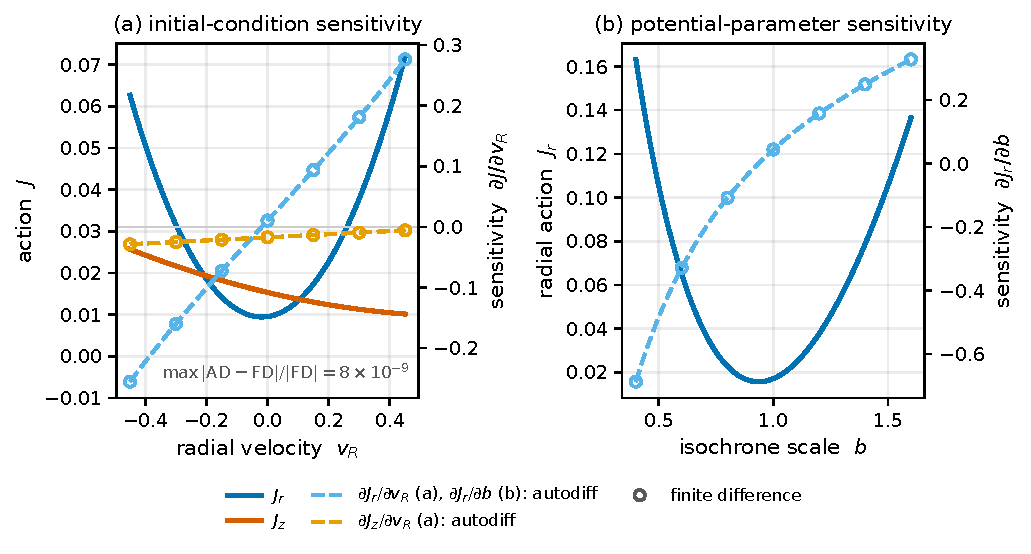
\includegraphics[width=\textwidth,clip=]{../figures/g18_actionangle_sensitivity/g18_actionangle_sensitivity.pdf}
  \caption{Derivatives of actions in the isochrone potential. Left: the
    radial and vertical actions of an orbit as a function of its radial
    velocity (solid, left axis) and their derivatives with respect to
    the radial velocity by automatic differentiation (dashed, right
    axis) with finite differences (circles). Right: the radial action as
    a function of the scale radius $b$ of the potential and its
    derivative with respect to $b$.}\label{fig:aasens}
\end{figure*}

\subsection{The St\"{a}ckel and adiabatic approximations}\label{sec:aa-staeckel}

\texttt{actionAngleStaeckel}, the workhorse for axisymmetric potentials,
has two implementations that behave differently under a backend. The
pure-\python\ path (\texttt{c=False}) was rewritten as part of this work
to be vectorized over phase-space points, where it previously looped
over them, and the same code runs under \numpy, \jax, and \torch: the
turning points are found by the fixed-count bisection and Newton
polish of \sectionname~\ref{sec:design-numerics}, and the action,
frequency, and angle integrals are evaluated with the same Gauss--Legendre
rule, in an anomaly variable that removes the square-root singularities
at the turning points, that the \cc\ implementation uses, such that the
two agree to machine precision. Everything on this path is
differentiable with respect to the phase-space coordinates and the
potential's parameters,
\begin{code}
def jr_of_a(a):
    aAS= actionAngleStaeckel(pot=MiyamotoNagaiPotential(a=a,b=0.3),
                             delta=0.4,c=False)
    return aAS(R,vR,vT,z,vz)[0].sum()
djr_da= jax.grad(jr_of_a)(0.5)
\end{code}
with the restriction that the derivative of the action integral is of
first order only. \figurename~\ref{fig:staeckelq} shows such a
derivative, of the radial and vertical actions of a Sun-like orbit with
respect to the flattening of a logarithmic halo, with the potential and
the St\"{a}ckel transformation rebuilt from $q$ inside the differentiated
function: the automatic derivative agrees with finite differences to
$10^{-10}$, at the bottom of the finite-difference error curve, and once
compiled it costs about a millisecond.

\begin{figure*}[t!]
  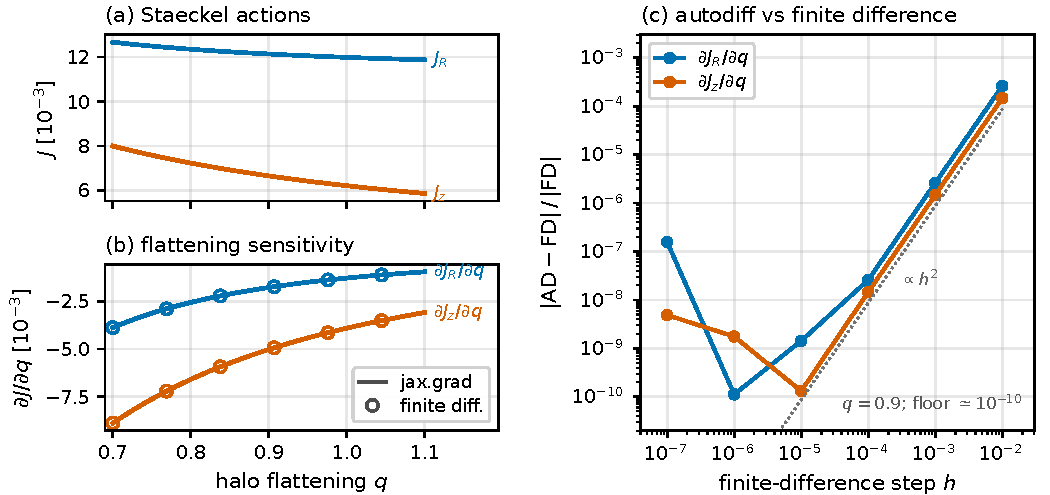
\includegraphics[width=\textwidth,clip=]{../figures/gA1_staeckel_param_sensitivity/gA1_staeckel_param_sensitivity.pdf}
  \caption{Derivatives of St\"{a}ckel actions with respect to a parameter
    of the potential. (a) The radial and vertical actions of a Sun-like
    orbit in a logarithmic halo as a function of its flattening $q$,
    computed with \texttt{actionAngleStaeckel(c=False)} at fixed focal
    length. (b) Their derivatives with respect to $q$ by \texttt{jax.grad}
    (lines) and by central finite differences in which the potential and
    the action--angle object are rebuilt (circles). (c) The relative
    difference between the two at $q=0.9$ as a function of the
    finite-difference step: the finite difference converges as $h^2$ onto
    the automatic derivative until rounding error takes over below
    $10^{-10}$.}\label{fig:staeckelq}
\end{figure*} The \cc\ path (\texttt{c=True}) is much faster for
small numbers of points and, on a backend, does more than before: the
\cc\ code computes, along with the actions, frequencies, and angles,
their Jacobian with respect to the five phase-space coordinates, and
this Jacobian is attached to the result as a custom derivative rule,
such that \texttt{jax.grad} or \torch's \texttt{backward} through a
\texttt{c=True} call costs one \cc\ call and a matrix product,
\begin{code}
aAS= actionAngleStaeckel(pot=MWPotential2014,delta=0.45,c=True)
def total_jr(R):
    return aAS(R,vR,vT,z,vz)[0].sum()
djr_dR= jax.jit(jax.grad(total_jr))(jnp.asarray([1.1,0.9]))
\end{code}
As for the orbit integrators, the \cc\ path gives derivatives with
respect to the phase-space position only, to first order, and the focal
length \texttt{delta} is a fixed number; derivatives with respect to the
potential's parameters require \texttt{c=False}. The estimate of the
focal length from the potential, \texttt{estimateDeltaStaeckel}, runs on
the backends and traces, such that a focal length estimated along an
integrated orbit can be part of a compiled program,
\begin{code}
delta= estimateDeltaStaeckel(MWPotential2014,o.R(ts),o.z(ts))
aAS= actionAngleStaeckel(pot=MWPotential2014,delta=delta,c=False)
jr,lz,jz= aAS(o.R(ts),o.vR(ts),o.vT(ts),o.z(ts),o.vz(ts))
\end{code}
The grid-based interpolated version,
\texttt{actionAngleStaeckelGrid}, builds its grid on the backend, such
that the grid lives on the GPU when the potential does and the
interpolated actions are differentiable with respect to the query
point; when the potential carries a parameter that is being
differentiated, the grid class delegates to the exact method, with a
warning, because the grid cannot be differentiated through its
construction. The adiabatic approximation follows the same pattern,
with a fused Jacobian in \cc\ for \texttt{c=True} and, for
\texttt{c=False}, the migrated spherical and vertical machinery for
its radial and vertical parts.

\subsection{Spherical potentials, the isochrone approximation, and the inverse transformation}\label{sec:aa-other}

The isochrone and harmonic-oscillator actions are closed forms and were
migrated by swapping the namespace. \texttt{actionAngleSpherical}
replaces its \scipy\ root finds and adaptive quadratures with the
shared root finder and a fixed-order Gauss--Legendre rule, with special
handling of circular and near-circular orbits, where the radial
integral degenerates, and of orbits that are unbound. The
\texttt{actionAngleIsochroneApprox} method of \citet{Bovy2014}
integrates an auxiliary orbit, and does so with the in-backend solvers
of \sectionname~\ref{sec:orbit-paths}; it is therefore differentiable
with respect to the potential's parameters, twice so under \jax\ with
the direct adjoint, and runs on a GPU.

The inverse transformation, from actions and angles to positions and
velocities, exists in \galpy\ for the isochrone and harmonic potentials
in closed form and for general one-dimensional potentials through
\texttt{actionAngleVerticalInverse}, which constructs a torus map by a
momentum-matched canonical transformation and tabulates it as a
function of the action. The construction---a root find for the maximum
excursion, a spectral sweep over the angle, a batched Gauss--Newton
solve for the anomaly, and Hermite-spline tables---and the evaluation
run natively on the backends, trace under compilation, and are
differentiable with respect to the action, the angle, and the
parameters of the potential, such that the family of tori can be
differentiated with respect to the parameters of the disk that
generates them. \figurename~\ref{fig:vinverse} demonstrates this for a
self-gravitating isothermal disk: the derivative of the tori with
respect to the velocity dispersion of the disk predicts the tori of a
nearby disk, agrees with finite differences to $10^{-10}$, and serves
as the Jacobian of a Levenberg--Marquardt fit of the disk's parameters to
stars scattered around three tori. In code, the tori of a family of disks
parametrized by their velocity dispersion are differentiated as
\begin{code}
def torus(sigma):
    disk= IsothermalDiskPotential(amp=1.,sigma=sigma)
    aAVI= actionAngleVerticalInverse(pot=disk,Es=Es,nta=128,
                                      setup_interp=True)
    return aAVI.xvFreqs(J,angles)[:2]  # (z, v_z) on the torus
z,vz= torus(0.5)
dz_dsigma,dvz_dsigma= jax.jacfwd(torus)(0.5)
\end{code}
The older construction modes of the
class, which use point transformations, are evaluated natively but
built on \numpy, and therefore cannot take a potential with backend
parameters.

\begin{figure*}[t!]
  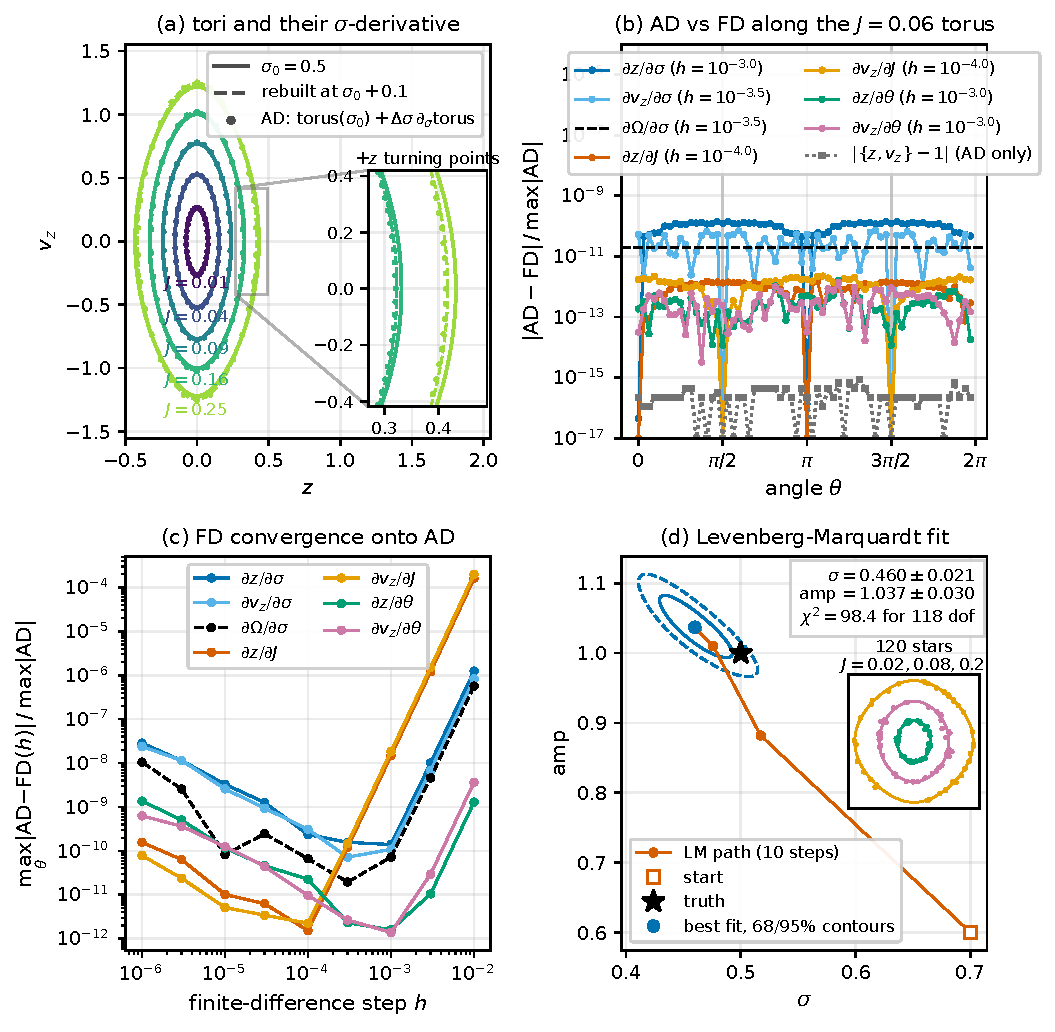
\includegraphics[width=\textwidth,clip=]{../figures/gV1_vertical_inverse/gV1_vertical_inverse.pdf}
  \caption{Differentiable inverse action--angle transformation in a
    self-gravitating isothermal disk with \texttt{actionAngleVerticalInverse}.
    (a) Tori at fixed actions for a disk with velocity dispersion
    $\sigma_0$ (solid), the same tori for a disk rebuilt with
    $\sigma_0+0.1$ (dashed), and the first-order prediction from the
    derivative of the tori with respect to $\sigma$ by automatic
    differentiation (points). (b) The difference between the derivatives
    of $z$, $v_z$, and the frequency with respect to $\sigma$, $J$, and
    $\theta$ along the $J=0.06$ torus and five-point finite differences,
    relative to the largest derivative. (c) The finite differences
    converge onto the automatic derivatives as $h^4$ until their
    round-off floor. (d) A Levenberg--Marquardt fit of $(\sigma,\,\mathrm{amp})$
    and 120 angles to 120 stars with noisy $(z,v_z)$ on three tori, using
    the automatic Jacobian; the fit converges in ten steps and the truth
    lies inside the 68\,\% contour.}\label{fig:vinverse}
\end{figure*}

\subsection{Speed}\label{sec:aa-speed}

Two things changed in the speed of the action--angle calculations. The
vectorized \python\ St\"{a}ckel path is now as fast as the single-threaded
\cc\ path for large numbers of points on the CPU, where the old
per-object loop was more than an order of magnitude slower, and this
holds for plain \numpy. And on a GPU, the same path under \torch\ or
compiled \jax\ overtakes the \cc\ path by an order of magnitude at
$10^5$ points, after a launch-bound floor of about a second; eager
\jax, which dispatches hundreds of small operations per call, is bound
by that dispatch and stays at a floor of several seconds. %TODO: Staeckel speed figure (g17) and its numbers after the re-measurement

The one-dimensional inverse transformation is shown in
\figurename~\ref{fig:vinvspeed}. Evaluating the torus map at $N$ angles
is fastest with \numpy\ for up to a few thousand angles, where the
backends pay their per-call overhead; compiled \jax\ overtakes it near
$N=10^4$ %TODO: 1-core jax CPU re-measurement (the current jax CPU series used up to 72 threads)
and on the H100 the same evaluation takes 11\,ms. The
backends find the angle with the same safeguarded Newton iteration as
\numpy, started at the requested angle. Constructing the map for a
family of $n_E$ energies is faster on every backend than on \numpy, by
an order of magnitude at $n_E=256$, because the batched Gauss--Newton
solve replaces a loop over tori; on a GPU the compiled construction takes
a few milliseconds whatever the size of the family. These numbers are for
the development machine and the H100 and should be read as orders of
magnitude.

\begin{figure*}[t!]
  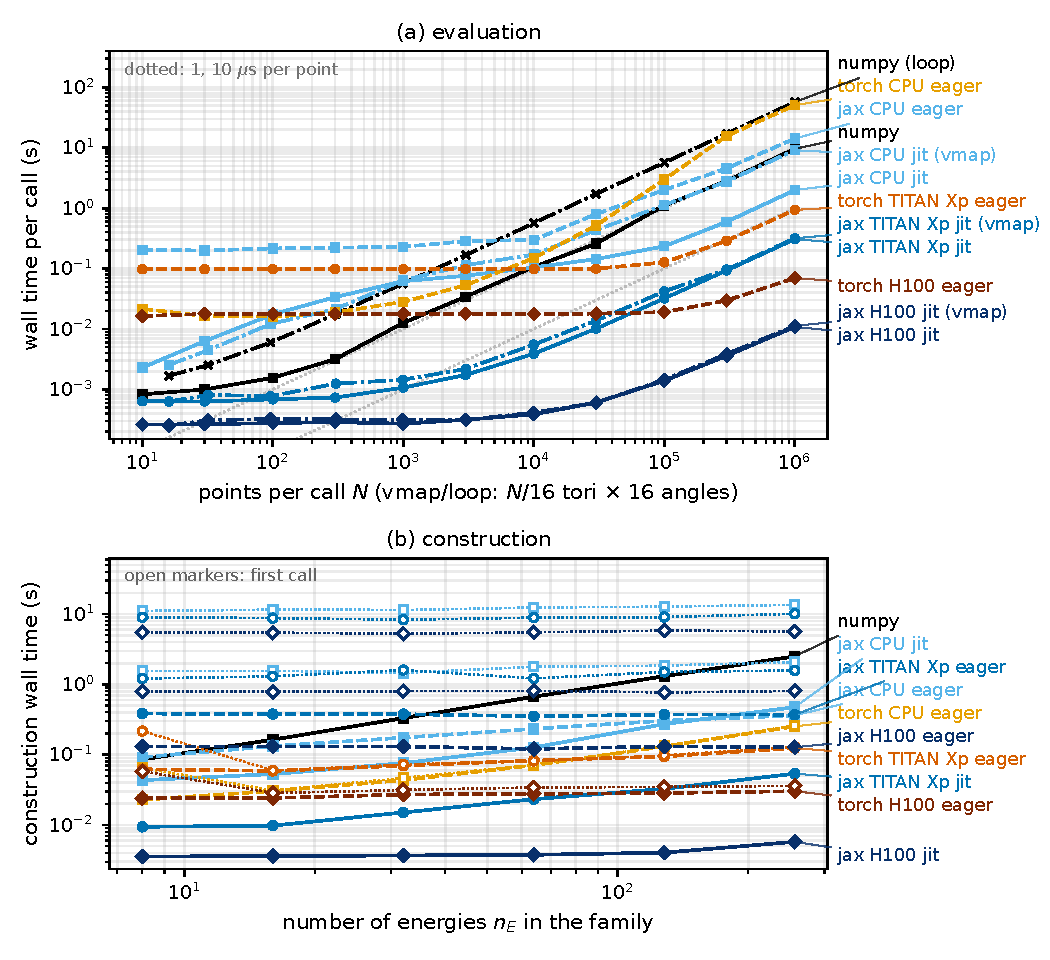
\includegraphics[width=\textwidth,clip=]{../figures/gV2_vertical_inverse_speed/gV2_vertical_inverse_speed.pdf}
  \caption{Speed of the one-dimensional inverse action--angle
    transformation, \texttt{actionAngleVerticalInverse}, for an
    isothermal disk. (a) Wall time to evaluate positions, velocities, and
    frequencies at $N$ angles on one torus (or, dash-dotted, at 16 angles
    on each of $N/16$ tori) with \numpy\ and on the backends on a single
    CPU core, the TITAN~Xp, and the H100; compilation time is excluded.
    (b) Time to construct the map for a family of $n_E$ energies, warm
    (filled markers) and on the first call (open markers), which for
    eager \jax\ includes compiling every operation for the new
    shapes.}\label{fig:vinvspeed}
\end{figure*}

\section{Distribution functions}\label{sec:df}

\subsection{General approach}\label{sec:df-general}

\galpy\ contains DF models to represent spherical and disky galactic components.
These DF models are constructed from a potential and a set of parameters,
they can be evaluated at phase-space points, integrated to obtain their moments 
(densities, mean velocities, and velocity dispersions), and they can be sampled.
On the backends, evaluation and the moments are differentiable for
every DF, sampling is differentiable wherever it is done by inverse
transformation, which is everywhere except for the many-position
velocity sampler of the quasi-isothermal disk DF and the samplers of
the two-dimensional disk DFs (\sectionname~\ref{sec:df-disk}), and
construction is differentiable for every DF whose construction is
itself a numerical computation---the spherical DFs obtained by
inverting a density, the King model, the quasi-isothermal disk DF,
whose table of guiding-center radii is then built on the backend, and
the stream models of \sectionname~\ref{sec:streams}. The parameters
of a DF, like those of a potential, can be given as backend arrays and
are then differentiated through everything that follows.

Every sampler in \galpy\ takes a \texttt{key=} argument:
\texttt{key=None} reproduces the previous behavior, drawing
from \numpy's global generator with the previous algorithm, while a
backend key selects the inverse-cumulative samplers of
\sectionname~\ref{sec:design-numerics} and returns backend arrays. For a
fixed key, the sample is then a smooth function of the DF's and the
potential's parameters, and its derivative is the pathwise, or
reparameterization, derivative: differentiating a statistic of the sample with respect to a
parameter gives an unbiased estimate of the derivative of the
expectation of that statistic. \figurename~\ref{fig:dfsample} shows an
explicit check that the pathwise derivative of a sample is the
derivative of the expectation, independently of any DF construction:
we differentiate a kernel estimate of the velocity dispersion over a
large fixed sample with respect to radius and compare with the
derivative of the Jeans equation; the two share no code and agree
within the Monte-Carlo noise. \figurename~\ref{fig:dfparam} then shows
the derivative of a sample through the construction of the DF, for an
Osipkov--Merritt DF of a Hernquist sphere constructed and sampled
inside a single compiled function of the scale radius: the derivative of
the sampled velocity dispersion with respect to the scale radius agrees
with the derivative of the Jeans-equation prediction to within the
Monte-Carlo noise, and with a finite difference of the same sample to
$10^{-7}$. The same figure shows the other kind of derivative of a DF's
construction, that of the King model's density profile with respect to
the dimensionless central potential $W_0$ at fixed mass and tidal
radius, which passes through the solution of the Poisson equation. In
eager mode, \galpy\ solves this ODE with \scipy\ and attaches the
derivative from the forward sensitivity equations, while under
compilation it solves the same ODE in the backend.

\begin{figure*}[t!]
  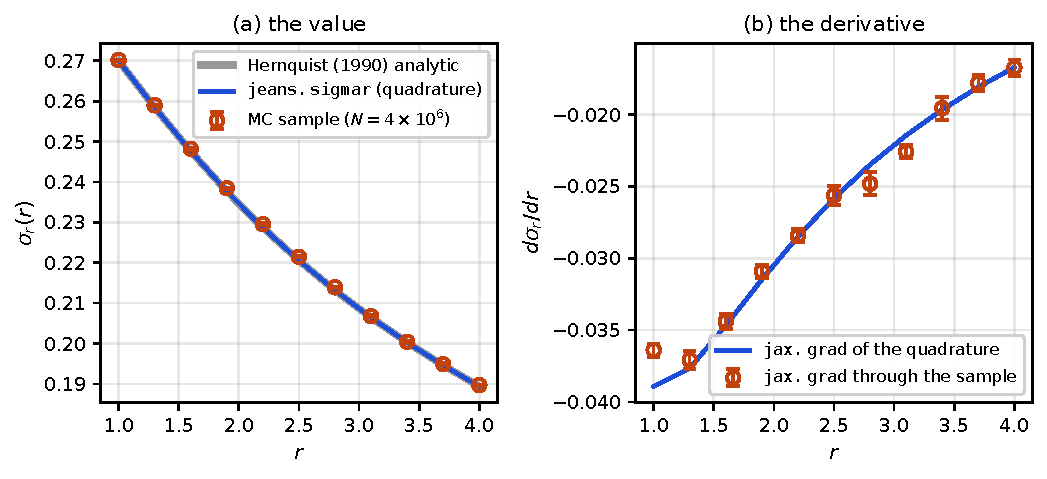
\includegraphics[width=\textwidth,clip=]{../figures/gD2_df_sample_autodiff/gD2_df_sample_autodiff.pdf}
  \caption{A derivative through a DF sample. Left: the radial velocity
    dispersion of the isotropic Hernquist DF from the analytic
    expression, from the Jeans equation by quadrature, and from a sample
    of $4\times10^6$ particles. Right: its derivative with respect to
    radius, from \texttt{jax.grad} of the Jeans quadrature and from
    \texttt{jax.grad} of a kernel estimator over the fixed sample, with
    error bars from eight sub-samples; the two agree to a median of
    $0.5\sigma$ of the Monte-Carlo noise, with the innermost point at
    $5\sigma$ from the bias of the kernel.}\label{fig:dfsample}
\end{figure*}

\begin{figure*}[t!]
  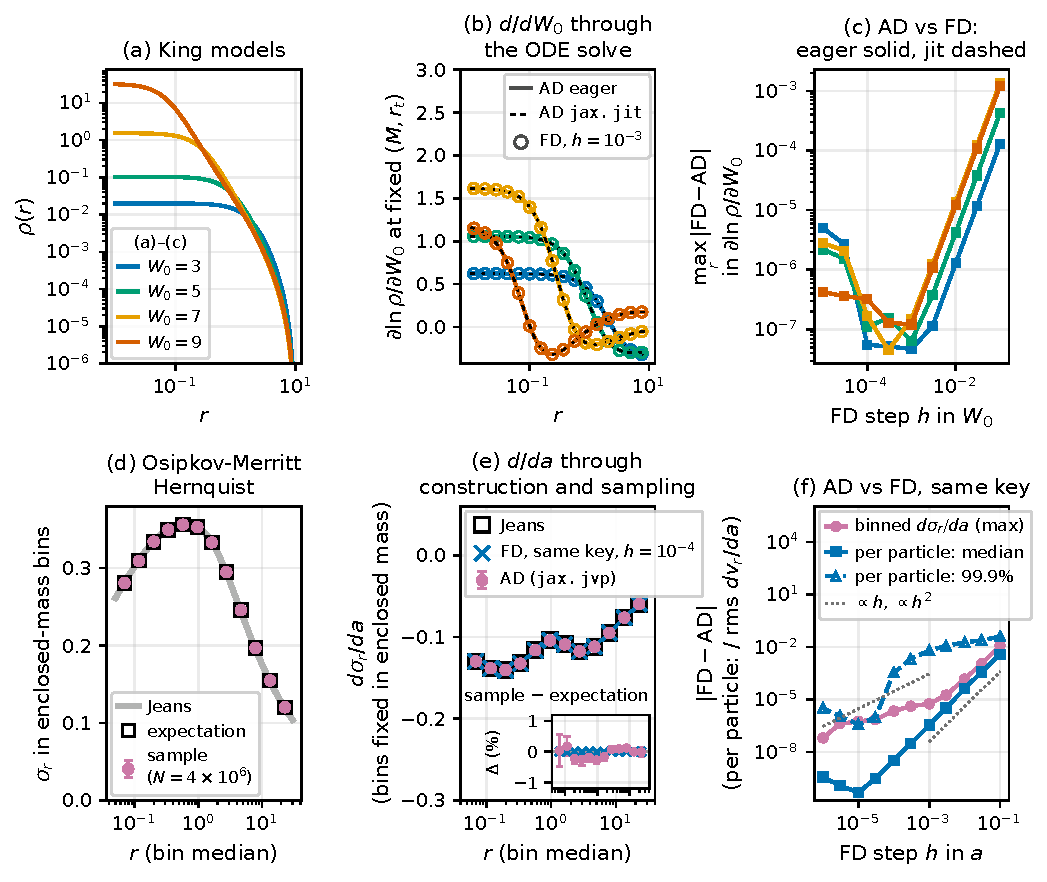
\includegraphics[width=\textwidth,clip=]{../figures/gD4_spherical_df_param/gD4_spherical_df_param.pdf}
  \caption{Derivatives through the construction and sampling of
    spherical DFs. Top row: (a) King models of unit mass and tidal radius
    $r_t=10$ for four values of $W_0$; (b) the derivative $\partial\ln\rho/\partial W_0$
    at fixed $(M,r_t)$ through the solution of the Poisson equation,
    eagerly with \scipy\ and under \texttt{jax.jit} with \diffrax, compared
    with a finite difference in which the model is rebuilt, and (c) the
    convergence of that finite difference onto the automatic derivative. 
    Bottom row: an Osipkov--Merritt DF of a Hernquist sphere with
    anisotropy radius $r_a=1.5$, constructed and sampled ($4\times10^6$
    particles) in one compiled function of the scale radius $a$; panel (d) shows that the
    sampled velocity dispersion matches the Jeans equation, (e) demonstrates that its
    derivative with respect to $a$ through construction and sampling
    matches both a finite difference of the same sample and the Jeans
    expectation within the Monte-Carlo noise, and panel (f) shows that the per-particle
    derivatives converge onto the automatic ones as $h$ and $h^2$.}\label{fig:dfparam}
\end{figure*}

\subsection{Spherical DFs}\label{sec:df-spherical}

The spherical DFs of \galpy---the Eddington inversion for isotropic
systems, the Osipkov--Merritt and constant-anisotropy inversions, the
King model, and the closed-form Hernquist and NFW DFs---share one
sampler, which draws radii by inverting the cumulative mass profile and
velocities by inverting a tabulated $p(v|r)$, and which on the backends
does both by interpolation in tables that are differentiable in their
knots. The inversions themselves, which are integrals of a derivative
of the density over the potential, use fixed-order Gauss--Legendre
quadrature in substituted variables and are differentiable through the
integrand, such that the DF can be differentiated with respect to the
parameters of the density and potential that it is built from. The
King model is the one DF whose \numpy\ result changed on purpose: its
Poisson equation is now solved to a relative tolerance of $10^{-10}$
rather than \scipy's default of $10^{-3}$, which left errors of order
$10^{-4}$ in its tables (\sectionname~\ref{sec:design-principles}). The
constant-anisotropy DF is the one place where \jax\ was already present
in \galpy, as an optional dependency for the fractional derivative in its
inversion; its construction is now much faster than it was, by about a
factor of four on \numpy\ and by orders of magnitude under
compilation, because the $f(E)$ inversion is a fixed-shape quadrature
that compiles well. As an example,
under \torch\ we obtain the derivative of a set of sampled radii with
respect to the scale radius of a Hernquist potential as
\begin{code}
a= torch.tensor(1.,dtype=torch.float64,
                requires_grad=True)
hp= HernquistPotential(amp=2.,a=a)
df= constantbetadf(pot=hp,beta=-0.2)
key= galpy.backend.random.key(7,backend='torch')
sam= df.sample(n=1000,key=key)
dr_da= torch.autograd.grad(sam.r().sum(),a)
\end{code}
and for a Hernquist sphere this derivative is $r_i/a$, which the sampler
reproduces to $10^{-13}$. Under \jax, construction, evaluation, and
sampling of these DFs run under \texttt{jax.jit}, and for the King
model so does the derivative with respect to $W_0$, as in for example
\begin{code}
def sigmar(W0):
    kdf= kingdf(W0=W0,M=2.3,rt=1.4)
    return kdf.sigmar(0.5)
dsig= jax.jit(jax.grad(sigmar)) # ODE by diffrax
dsig(3.)
\end{code}
A DF built from a density that is not the one generating the
potential is differentiable with respect to the parameters of both the
density and the potential; for example, with respect to those of the
density:
\begin{code}
def dispersion(a_tracer):
    hp= HernquistPotential(amp=0.1,a=a_tracer)
    df= eddingtondf(pot=NFWPotential(amp=1.,a=2.),
                    denspot=hp)
    return df.sigmar(1.)
jax.grad(dispersion)(0.7)
\end{code}
The closed-form DFs, including the analytic DFs of \citet{Evans1997}
for power-law spheres, and the energy derivative of their mass
profiles are likewise differentiable.

\subsection{Disk DFs}\label{sec:df-disk}

\galpy\ contains models for two-dimensional and three-dimensional disk DFs.
The two-dimensional axisymmetric disk DFs of \citet{Dehnen1999},
\citet{Shu1969}, and Schwarzschild
and their moments are evaluated with nested Gauss--Legendre quadrature
on the backends and are differentiable with respect to the parameters of
their surface-density and velocity-dispersion profiles; their samplers,
which draw by rejection, remain \numpy\ code, and we did not migrate
the corrections of these DFs for the difference between their input and
output profiles. \galpy\ also contains 
a two-dimensional non-axisymmetric disk DF that is a perturbation of a Dehnen DF by a
non-axisymmetric and/or time-dependent potential, which is evaluated by integrating orbits
backwards in time to an initial axisymmetric DF (in \texttt{galpy.df.evolveddiskdf}). 
The moments of
this evolved disk DF differentiate through that integration,
which on the backends is one vectorized in-backend solve over the
velocity grid rather than a loop. 

As a three-dimensional disk DF, \galpy\ implements the quasi-isothermal
DF of \citet{Binney2010,BinneyMcMillan2011}, in the form used by
\citet{BovyRix2013},
which is a function of the actions and is evaluated by first computing the actions with 
\texttt{actionAngleStaeckel} and then evaluating the DF.  The quasi-isothermal DF is now 
evaluated and its moments computed on the backends,
differentiably with respect to the parameters of the potential and the
DF's scale lengths, and its velocity sampler at a given position draws
by inverse transformation on a three-dimensional velocity mesh, such
that a sample drawn with a fixed key is a differentiable function of the
DF's parameters;
this sampler replaced a rejection sampler on the \numpy\ path as well,
which is one of the two places where the \numpy\ draws changed (the
distribution is the same, the particular draws are not). In code this looks as follows:
\begin{code}
qdf= quasiisothermaldf(1./3.,0.2,0.1,1.,1.,
                       pot=MWPotential2014,aA=aAS)
vs= qdf.sampleV(0.9,0.05,n=10**4,
                key=grandom.key(0,backend='jax'))
sigma_R= jnp.std(vs[:,0])
\end{code}
Its construction tabulates the guiding-center radius as a function of
angular momentum, which is built on the backend when the potential or a
scale length carries a backend parameter, such that the DF and its
moments are differentiable through the construction. Its interpolated
velocity sampler, which samples many positions at once, is a rejection
sampler with \numpy\ proposals that runs on the backends, with its
shrinking arrays padded to fixed sizes, but is not differentiable.

\subsection{Speed}\label{sec:df-speed}

Sampling is where the backends change what is practical, as is clear
from \figurename~\ref{fig:dfspeed}, which displays the time to draw $N$
particles from four spherical DFs. On the CPU, eager \jax\ and \torch\ are slower
than \numpy\ for small samples, because every one of the hundreds of
array operations in a draw is dispatched separately and each costs a few
to tens of microseconds, and they catch up only at $N\approx10^4$;
compiled \jax\ is faster than \numpy\ at every size, by a factor of
1.5 to 6 at $N=10^7$ on one core, because the compiler fuses the
hundreds of array operations of a draw into a few loops, where \numpy\
executes each separately and writes its intermediate results to
memory. On a GPU the sample of $10^7$ particles takes
tens of milliseconds on the consumer card and a few milliseconds on the
H100, two to nearly four orders of magnitude faster than \numpy\ on
one core. The lower panel
shows the cost of constructing a DF, which for the inversions is
dominated by the $f(E)$ integral: more than a minute on \numpy\ for the
constant-anisotropy DF, a fraction of a second once compiled, with the
compilation itself costing seconds and paid once.

\begin{figure*}[t!]
  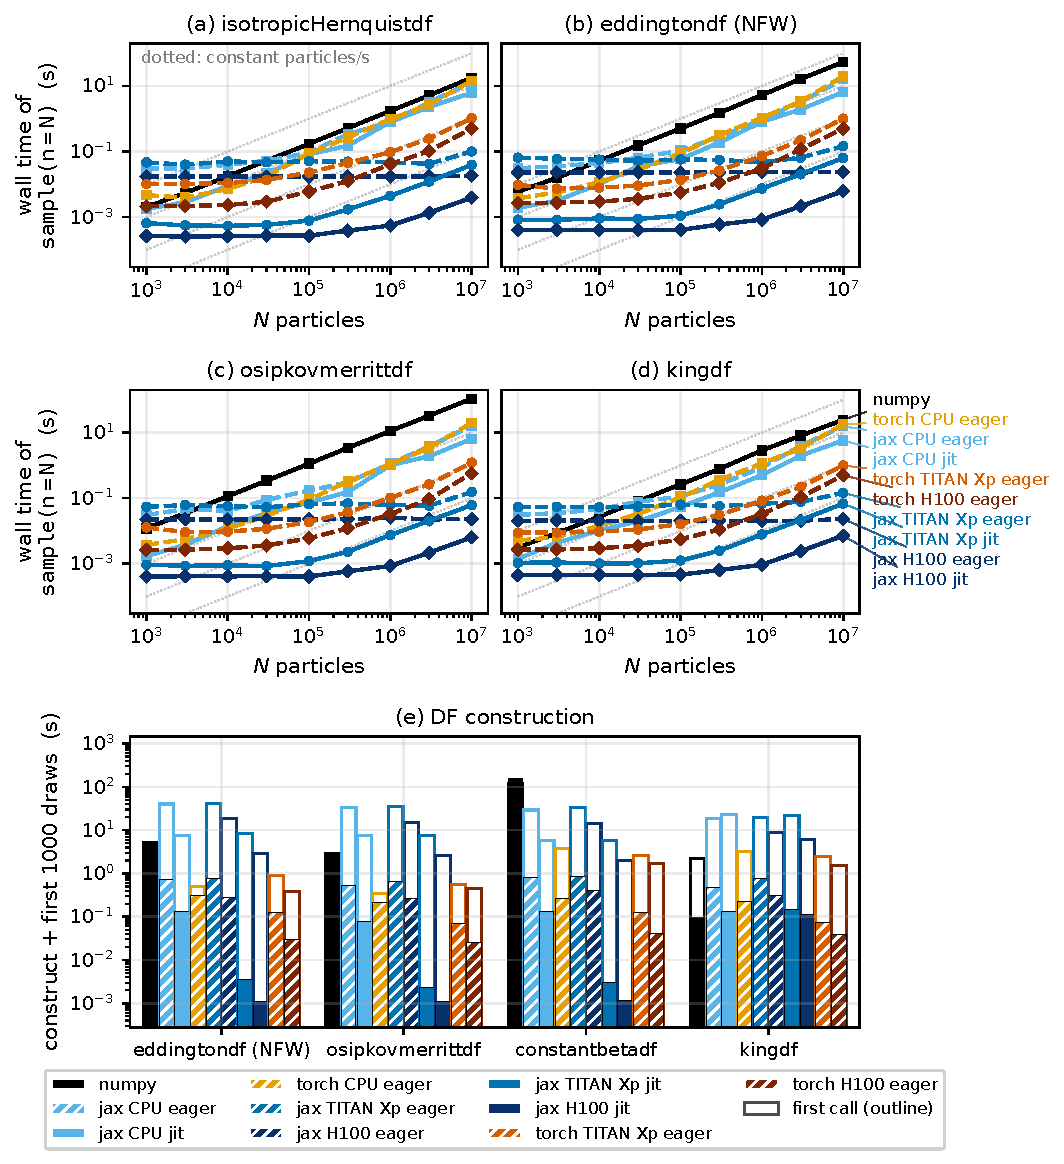
\includegraphics[width=\textwidth,clip=]{../figures/gD3_spherical_df_speed/gD3_spherical_df_speed.pdf}
  \caption{Speed of sampling and constructing spherical DFs. Top: wall
    time of \texttt{sample(n=N)} for the isotropic Hernquist DF, the
    Eddington inversion of an NFW profile, an Osipkov--Merritt DF, and a
    King model, on \numpy\ and on the backends on the CPU, the TITAN~Xp,
    and the H100; solid lines are compiled, dashed eager. Bottom: time to
    construct each DF and draw a first thousand particles, warm (filled)
    and including compilation on the first call in a fresh process
    (outline); hatched bars are eager. All CPU series use one core. Compiling with \texttt{jax.jit} or
    running on a GPU makes sampling much faster than with \numpy, by two
    to nearly four orders of magnitude on a GPU for large samples.}\label{fig:dfspeed}
\end{figure*}

\section{Tidal streams}\label{sec:streams}

Tidal streams are the application for which \galpy's DFs are most often
fit to data, and the one in which derivatives have been most sorely
missed, because a stream model is an expensive forward computation with
a handful of parameters, the potential's among them, and fitting it has
meant exploring that parameter space with a sampler that knows nothing
of the model's smoothness. \galpy\ contains three stream models, all of
which now run on the backends: the action--angle model of
\citet{Bovy2014}, \texttt{streamdf}, with its extension to stream gaps
\citep{Sanders2016}; and the particle-spray models of \citet{Fardal2015}
and \citet{Chen2025}, \texttt{streamspraydf}.

\subsection{The action--angle stream model}\label{sec:streams-streamdf}

\texttt{streamdf} models a stream as a distribution in frequency and
angle space, computes the mean track of the stream in configuration
space by iterating the transformation between the two, and samples and
evaluates the DF around that track. On the backends the track
computation is a pure function of the progenitor's orbit and the
potential that is vectorized over the segments of the track and is
differentiable from end to end: the auxiliary orbits are integrated in
the backend, and the Jacobian of the action--angle transformation along
the track, which was a finite-difference Jacobian in the \numpy\ code,
is the automatic Jacobian of the methods of \sectionname~\ref{sec:aa}.
The derivative of the track with respect to a parameter of the
potential agrees with a finite difference of the same computation to a
few parts in $10^4$, which is the level set by the fixed iteration count
of the track refinement. Construction of a \texttt{streamdf} is
differentiable with respect to the potential, and can be compiled,
although the compilation of a construction, which contains tens of
orbit integrations and the iteration of the track, takes a quarter of an
hour and is only worthwhile when many streams are to be built; the
construction itself, once compiled, takes about a minute on a CPU,
compared with a few to tens of seconds for the \numpy\ and \cc\ version.
Sampling and evaluating the DF, on the other hand, are two orders of
magnitude faster under compilation than on \numpy, and run on a GPU.

A point about these derivatives is general enough to state here. A
stream model is a generative model: the stream's stars are a sample from
the model's DF. The derivative of the track with respect to a parameter
can be taken with the sample of stars held fixed, which is what one
obtains by differentiating the track code alone, or by letting the
sample move with the parameter, which is what a finite difference of the
full model computes. The first is not a physical quantity, and the two
differ. Where \galpy\ provides derivatives of stream models, they are of
the second kind, and they are tested against finite differences whose
step is shown to be converged.

\subsection{Particle-spray models}\label{sec:streams-spray}

The particle-spray models release particles from the progenitor at
random times with random offsets in position and velocity and integrate
them forward. On the backends, \texttt{sample()} and the track-fitting
method \texttt{streamTrack()} are pure functions of the progenitor's
orbit, the potential, the progenitor mass (or a mass history), and a
random key: the stripping times are drawn by inverse transformation of
uniform variates, the offsets by reparameterized normal variates, the
progenitor and the particles are integrated in the backend, and the
track is fit with a penalized spline. The whole computation compiles
and is differentiable with respect to every parameter,
\begin{code}
key= galpy.backend.random.key(1,backend='jax')
def leading_arm(q):
    spdf= fardal15spraydf(mass,progenitor=Orbit(ic),tdisrupt=4.5/time_in_Gyr(),
                          pot=LogarithmicHaloPotential(normalize=1.,q=q))
    return spdf.sample(n=1500,return_orbit=False,tail='leading',key=key)
track_and_dtrack= jax.jvp(leading_arm,(q0,),(1.,))
\end{code}
where the forward-mode derivative gives the change of every particle's
position for a unit change in the halo flattening, with the random
numbers in common between the two. The derivative of the sampled stream
with respect to the potential agrees with finite differences of the same
sample to $10^{-6}$, and \figurename~\ref{fig:extrapolation}
demonstrates what it is good for: a single pass of forward-mode
differentiation over a 1500-particle stream predicts the stream's track
in a halo of different flattening well enough to remove most of the
shift in the track for changes in the flattening of up to twenty
percent, which is the kind of step a fitter takes. Each spray
particle's orbit is one more orbit in a batch, such that a sprayed
stream costs about a millisecond per particle on a CPU under compiled
\jax, about half the cost of the non-differentiable \cc\ version, and
microseconds per particle on a GPU (\figurename~\ref{fig:spraysp}).

\begin{figure}[t!]
  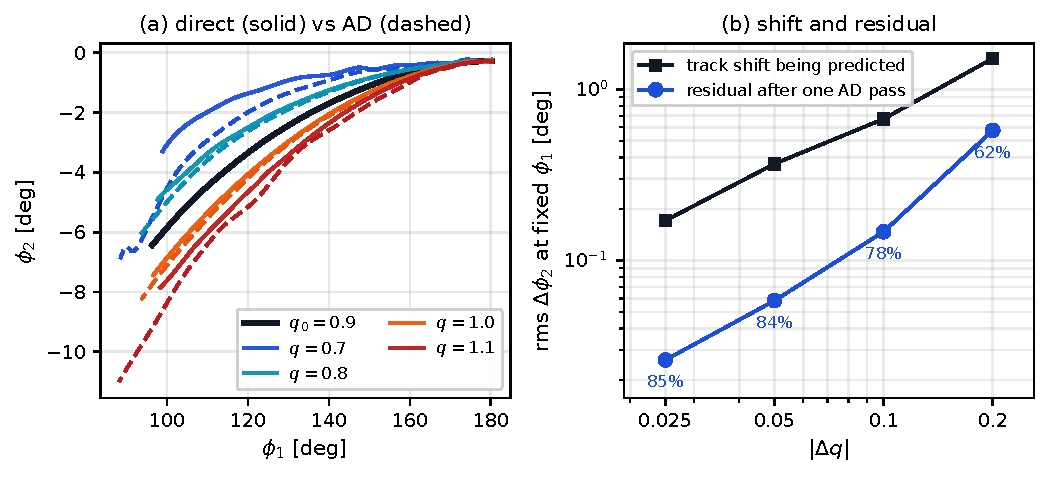
\includegraphics[width=0.48\textwidth,clip=]{../figures/gS3_track_extrapolation/gS3_track_extrapolation.pdf}
  \caption{Predicting a stream's track in a different potential from one
    derivative. Left: the track of a 1500-particle \texttt{fardal15spraydf}
    stream after 4.5\,Gyr in a logarithmic halo with flattening
    $q_0=0.9$ (black), the tracks in halos with $q=0.7$ to $1.1$
    computed directly (solid), and their prediction from the forward-mode
    derivative of the stream with respect to $q$ at $q_0$ (dashed), in a
    coordinate frame aligned with the progenitor's orbit. Right: the
    root-mean-square shift of the track at fixed $\phi_1$ and the
    residual after the first-order prediction, as a function of
    $|\Delta q|$.}\label{fig:extrapolation}
\end{figure}

\begin{figure*}[t!]
  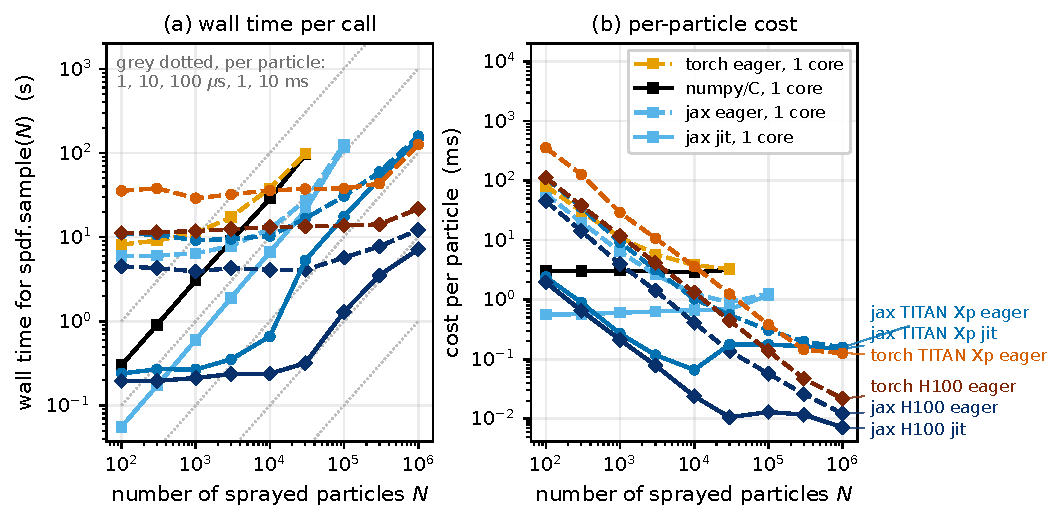
\includegraphics[width=\textwidth,clip=]{../figures/gS5_streamspray_speed/gS5_streamspray_speed.pdf}
  \caption{Speed of the particle-spray stream model: wall time (left)
    and cost per particle (right) of \texttt{fardal15spraydf.sample(N)}
    with 4.5\,Gyr of stripping, for the \numpy\ version with the \cc\
    integrator and for the differentiable backend version on the CPU,
    the TITAN~Xp, and the H100, compiled (solid) and eager
    (dashed).}\label{fig:spraysp}
\end{figure*}

\subsection{Stream gaps}\label{sec:streams-gaps}

The stream-gap model of \citet{Sanders2016}, \texttt{streamgapdf},
computes the velocity kick that a passing subhalo imparts along a stream
and propagates it through the action--angle model. The kick kernels for
the Plummer and Hernquist subhalos, the interpolation of the kicks along
the stream, and the transformation to the impact frame run on the
backends and are differentiable with respect to the parameters of the
impact, and the orbit integrations in the model go through the batched
in-backend solver when given backend inputs. The construction of the
model is not traceable, because it assigns into arrays in place in
many places, and this was left as it is.

\section{How the backends were built}\label{sec:process}

We carried out this work in a way that differs enough from how \galpy\
was developed before that we describe it in a section of its own.
Because an AI agent wrote the code, the question of how one comes to
trust such code is as much a part of this paper as the code itself. In
this section, we describe the organization of the work, how we reviewed
it, the stretch during which the agent worked without supervision, how
we made the existing test suite pass under the new backends, and the
checks through which we established that the code is correct. Because the division of labor between the human author and the
agent is the subject here, this section names them separately, as JB
and the agent.

\subsection{Organization}\label{sec:process-organization}

Work started on 2026 June 1 with a design discussion between JB and
Claude, Anthropic's AI coding agent, used through the \texttt{Claude
  Code} environment, which has access to a shell, to the \galpy\
repository, and to \github. The discussion settled the scope (all of
\galpy, on both \jax\ and \torch) and the constraints described in
\sectionname~\ref{sec:design}: byte-identity of the \numpy\ path, an
unchanged interface, no compilation inside \galpy, and the existing test
suite as one of the main acceptance tests. Passing the suite was not the
only goal: the coverage of the code by the tests was not to decrease
either (see the rules below). The first code, which took a day to
write, was a pilot that made two potentials run under all three array
libraries and checked value parity, gradients against finite
differences, and the identities between the potential, its forces, and
its second derivatives under automatic differentiation.

The work was organized in branches of the \galpy\ repository. \galpy's
main branch, from which version~1.x is released, continued to receive
its usual maintenance, as well as the fixes to the existing \numpy\ and
\cc\ code that the backend work turned up, which we always made there
first (\sectionname~\ref{sec:process-fixes}). The backend code was
developed on a long-lived \emph{backend branch}, to which every backend
change was proposed as a pull request (PR), either directly or through a
short-lived branch of its own when a change was split into several PRs.
The backend branch is periodically rebased onto the main branch, without
merge commits, so that it always contains the main branch's fixes, and it
becomes \galpy's version~2, released as pre-releases while the main branch
continues for now as version~1.x. The three-dimensional variational
equations had their own branch, which was merged into the main branch,
and during the stretch described in
\sectionname~\ref{sec:process-autonomous} the agent worked on a separate
development branch.

Between 2026 June 1 and October 30, 723 PRs were opened for this work,
of which 696 were merged: 602 on the backend branch and its sub-branches,
29 for the three-dimensional variational equations, and 65 against
\galpy's main branch, of which 40 fixed defects in the existing \numpy\
and \cc\ code that the backend work had found
(\sectionname~\ref{sec:process-fixes}), 16 added capabilities or
speed-ups to that code that came out of the work, and 9 concerned the
tests and the continuous integration. The merged PRs have a median size
of 182 changed lines (quartiles 74 and 372 lines).
We kept the size small on purpose, because a PR is reviewable when it
does one thing, and a backend migration of one module, with its tests,
is one thing. We split larger pieces of work into stacks of dependent
PRs that are reviewed in order (101 of the PRs are members of such stacks);
for example, we split the migration of the spherical DFs by DF family
into a base PR and four PRs that each port one family, and the port of
the one-dimensional inverse action--angle code into three. Each PR
carries a description of what was changed, the measurements that
support it (timings, parity counts, gradient errors), and what was
explicitly left out, such that the description can be reviewed without
re-deriving it from the diff.

The rate of PRs varied with the kind of work: in June, 88 backend PRs
and 29 PRs for the three-dimensional variational equations were opened
as the agent migrated the potentials family by family, in parallel, from
a fixed template. July was the peak, with 176 backend PRs: the agent ported the orbit,
action--angle, and DF modules, the autonomous stretch started, and the PRs were small, one problem each. In August (114) and
September (112), the work turned to the compiled modes, the test ledger
of \sectionname~\ref{sec:process-ledger}, and
the harder DFs, with PRs that were fewer and larger, because the
remaining problems were coupled; October, the last month of the
work, added 135 through the 30th.
Over the same months, the repository received a separate stream of 58
PRs in August and September for another \galpy\ project, which shared
the continuous integration and matters for the costs below.

In round numbers, the work cost the following. The agent ran on a
fixed-price subscription to Anthropic's Claude: until 2026 June 25 the
``Max'' plan at its 20$\times$ tier, which Anthropic provided free of
charge, afterwards the 5$\times$ tier at about CAD~140 per month, and
for the final two weeks the 20$\times$ tier again.
Successive versions of the Claude Opus models did the coding, while
Claude Fable was used only to draft this paper and its major revisions.
The far larger cost was
the continuous integration, because every backend PR runs \galpy's test
suite in five modes over 22 shards, about 150 jobs of 20 to 90 minutes
each; the GitHub Actions bill for the repository at list price was
\$13,100 in June, \$16,500 in July, \$15,800 in August,
\$10,200 in September, and \$8,600 in October 2026. June,
July, and October were almost entirely this project; in August and
September the backend PRs were about three quarters of the PRs and, since a PR to
the main branch runs only the \numpy\ suite, a larger fraction of the
compute, such that about \$59,000 of the total is attributable to the
backend project. GitHub's Education program covered
this cost, which would otherwise have been prohibitive. The continuous
integration was crucial to establishing that the PRs were correct: it
ran every test in every mode on every PR, and it often turned up errors
that the local runs before pushing had not, in modes, shards, or
versions of the dependencies that the agent had not tried. It was also
the bottleneck of the project, because a PR could not be merged
before its matrix had run, the shards queued behind each other when
several PRs were open, and a flaky job meant a two-hour wait. We made
several of the engineering decisions---cancelling the runs
of superseded commits, running the compiled modes only on demand until
they were stable, running the touched tests under forced backends
locally before pushing---to spend less time in that queue. \github's
support for stacks of dependent PRs, which rebases the members of a
stack and retargets them as the lower ones merge, arrived only on 2026
July 30. Before then, we based dependent PRs on each other's branches by
hand, and several open PRs that touched the same files had to be rebased
onto each other by hand every time one of them changed or merged, each
rebase triggering a new run of the whole matrix; the stacks removed most
of that work.

JB fixed a few rules early and enforced them throughout. The \numpy\ path
had to remain byte-identical, and any deviation (\sectionname~\ref{sec:design-principles}
lists them) was flagged in the PR rather than absorbed.
The \jax\ and \torch\ paths had to pass the same tests at the same
tolerances; a tolerance could be loosened only for one test, only
slightly, and with a justification in the PR. Test coverage was not
allowed to decrease, not by a single line; in the end, the backend
branch leaves 14 of its 56,950 executable statements uncovered, against
24 of 41,704 on the main branch. Tests had to make meaningful assertions
at tight tolerances: values had to match their reference to a relative
$10^{-13}$ or better, often $10^{-14}$, and derivatives a finite
difference that is shown to converge; a test could never merely check
that a result is finite, and only tests of sampling had looser
tolerances, set by their Monte Carlo noise. A test that
passes under a backend only because the code silently fell back to
\numpy\ does not count, and the agent hunted down such \emph{numpy
islands} specifically (\sectionname~\ref{sec:process-islands}). Before
pushing any PR, the agent ran its tests locally under forced \jax\ and
\torch\ backends, which the \numpy-only checks cannot do, and measured
the \numpy\ byte-identity by comparing checksums of outputs between two
checkouts that differ only in the files of the PR.

\subsection{Review}\label{sec:process-review}

Every PR was reviewed before it was merged into the backend branch, and
JB merged all of them except during the stretch described in
\sectionname~\ref{sec:process-autonomous}, whose work JB reviewed before
it was merged into the backend branch. Much of the review was
conversational, in the session in which the agent worked, and
concerned design as much as code: that a hand-rolled root finder
belongs in a utility module or should be replaced by \scipy's, that
speed-ups are to be demonstrated by timing both versions rather than
asserted, that tests should go through public methods rather than
internal functions, and so on. Reviews on \github\ itself caught the
kinds of problems that reviews of human code catch: a variable omitted
from an OpenMP \texttt{private} clause, a coverage drop of one line that
the automated check had passed.

Claude Code records every message of a session, and the token counts of
every response, in a transcript, from which we can estimate how much
input the work took. This is an estimate, not an exact count, because
separating JB's own text from the material that he passed on (reports
from other agents, reviews, logs) relies on simple heuristics. Between
2026 June 4 and October 30, JB sent about 2,500 messages, on 141 of the
149 days, almost a quarter of them while the agent was working, which
then folded them into the task at hand. Most were short, with a median
length of 14 words, and in total they contain about 57,000 words of
JB's own text, or roughly 110 single-spaced pages, plus about 33,000
words that he passed on. Over the same period, the agent produced about
114 million output tokens (including its reasoning and its tool calls;
a third of them in subagents that it started) and read about 44 billion
input tokens, almost all of them its own context re-read from a cache at
every step; these numbers do not include the other agents whose reports
JB passed on. Review on \github\ itself was light by comparison: of the
494 PRs that the agent opened under its own account (from July 26 on),
JB left a formal review on 23 and comments on 24.

JB also used two other forms of review. First, at several points he ran
an independent AI code reviewer (OpenAI's Codex) over the agent's work and
passed its findings to the agent to address, usually by pasting them into
the conversation (18 reviews in all). These reviews
found real defects: a gradient of the incomplete gamma function that
was \texttt{nan} at the endpoint $x=0$ although its value was correct;
a quadrature routine documented as accepting arrays that was correct
only for scalars; a surface-density routine that used the backend
quadrature only when the height above the plane was traced, such that a
derivative with respect to the radius at fixed height fell back to
\scipy\ and failed; and a branch-selection rule in the compiled path of
the hypergeometric function that returned infinity where the eager path
was correct. The agent reproduced each finding before fixing it and
dropped the findings that it could not reproduce with a note saying why.
Second, before merging complex PRs, JB instructed the agent to run
adversarial reviews of its own work by independent agents whose only
task was to break the PR against the real code; these found, for
example, that a stream sampler handed the same random key to the
position- and velocity-angle samplers, and that the parity tests of an
early PR compared at a tolerance four orders of magnitude too loose to
catch the $10^{-16}$ differences from re-associated arithmetic. The
latter finding set the pattern for all subsequent work: the original
\numpy\ expression is kept byte-for-byte and only the branching is
rewritten, never an algebraically equivalent form.

\subsection{The autonomous stretch}\label{sec:process-autonomous}

From 2026 July 26 to August 9, JB was away on vacation and the agent worked on its
own, with the goal of making the whole existing test suite pass under
compilation and of emptying the ledger of expected failures. For this,
the agent opened PRs against a separate development branch, which it
merged itself once the continuous integration was green, under the
understanding that JB would review the accumulated branch on his return.
It could not merge into the backend branch or into \galpy's main
branch, and it could not change the continuous-integration
configuration. These were hard guardrails rather than instructions: the
agent worked through its own \github\ account, which was set up for this
purpose and whose access token lacks the permission to modify the
workflow files that define the continuous integration, and branch
rulesets on \github\ allow changes to the main and backend branches only
through PRs that pass the required checks and, for the duration of the
stretch, blocked all updates of these two branches. A scheduler woke the agent at regular intervals to ensure
that it kept going, and the agent kept a dated log of what it did and
why; this log, which runs to 60,000 lines for the summer, is part of the
repository that accompanies this paper.

In the two unsupervised weeks, the agent merged 74 PRs. JB was pleased
enough with the progress on his return that he let the unsupervised
procedure continue for a few more weeks, alongside his supervised work,
and 145 PRs in total went through the development branch before it was
merged into the backend branch on 2026 September 2, after JB had
reviewed it as a whole and with the help of a Codex review (the
latter's verdict, that ``the work is coherent, the ledger is honest,''
matched JB's own). The stretch
made clear both what such an agent can and cannot do. It burned the
compiled-mode ledger down from 100 to 15 failing tests in three days,
found and fixed a performance problem in the coercion of inputs that had
cost 178\,$\mu$s per call, resolved the interaction between
\astropy\ units and compilation, and found two pre-existing bugs in
\galpy's \numpy\ code that it validated against a 30-digit reference
before filing them as issues. It also introduced regressions, all of
which it found itself within days using the tools it had built for the
purpose---a traced sweep of the suite, a comparison of test durations
between runs---and fixed before JB returned; it misread a stale rule;
it once left conflict markers in a working tree, the type of error that
a human review would have spotted easily; and its summary table
of PRs fell out of date and had to be rebuilt from \github. The
scorecard that it wrote for itself judged the stretch against its goal
honestly: the ledger went from 392 to 140 entries against a target of
zero. We have kept this account in the paper because it is the kind of
information that a reader deciding whether to work this way needs. On
the whole, the autonomous stretch succeeded in keeping the agent working
productively while JB was away, but it did so because the agent had a
clear, limited, and verifiable goal---emptying the ledger---and work
towards the broader aims of the project, which require judgment about
what to build and how, would have been much harder to leave unsupervised.

\subsection{Making the test suite pass under every backend}\label{sec:process-ledger}

One of the main acceptance tests for the backends was \galpy's own test
suite, run under \numpy, under \jax\ and \torch\ in eager mode, and
under \jax\ and \torch\ with compilation at every entry point, for a
total of five modes. Leaving aside the 27 tests of the out-of-scope
torus-mapping code (below), the suite grew from 2,462 to 4,462 tests
over the course of this work, mainly because we split existing tests
up: tests that looped over all of \galpy's potentials inside a single
test, for example, became one test per potential, such that each
failure and success could be traced to its potential. We did not delete
or modify tests that failed under a backend, but listed them in a
\emph{ledger}, one line per test and mode, that marked them as expected
failures, such that the size of the ledger was the measure of what
remained to be done. A second ledger listed tests that passed under a
backend but exceeded the time limit that we set for a single test in
the continuous integration, 300\,s, which keeps one hung or pathologically
slow test from stalling a shard of the matrix, and a third lists the
tests of code that is permanently out of scope. We regenerated the
ledgers from the actual test results on demand, such that they could
not drift from reality, and the continuous integration posted a report
of each PR's results per file and mode, ledgered failures included, to
the PR, such that a reviewer saw at a glance what a PR fixed or broke.
In addition, we ran a dedicated set of tests of the backend code itself,
now 18,807 tests in 100 files.

\begin{figure*}[t!]
  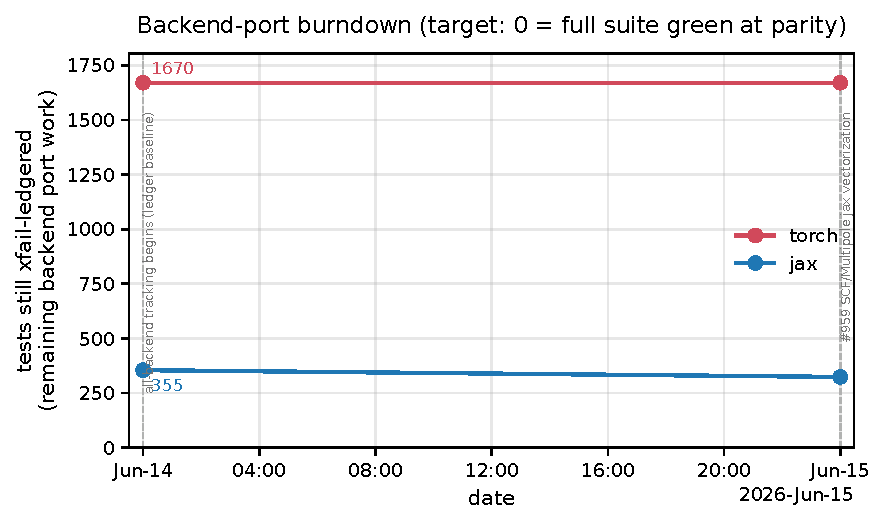
\includegraphics[width=\textwidth,clip=]{../figures/g13_ledger_burndown/g13_ledger_burndown.pdf}
  \caption{Tests of \galpy's existing test suite that pass under each
    backend, as a function of time, leaving aside the 27 tests of the
    out-of-scope torus-mapping code. The grey line is the size of the
    suite, which grows from 2,462 to 4,462 tests over the period (most
    of the jump on June 19 comes from splitting the potential tests into
    one test per potential); the colored curves show the number of these
    tests that pass under \torch\ (top) and \jax\ (middle) in eager mode
    (solid) and under compilation (dashed), that is, the size of the suite
    minus the tests that are ledgered as expected failures or as too slow,
    or skipped, under that mode, which is the shaded band. The compiled
    mode's ledgers are counted with the rules that the test configuration
    applied at each date; in August, \jax\ passes more tests under
    compilation than in eager mode because slow orbit tests that are
    skipped in eager mode run in reasonable time when compiled. The bottom
    panel shows the number of tests in the dedicated backend test
    modules; its jump in October is the two sweeps of
    \sectionname~\ref{sec:process-correctness}, which add 7,045
    parametrized cases. At the end, all 4,462 tests pass in every
    mode.}\label{fig:ledger}
\end{figure*}

\figurename~\ref{fig:ledger} displays how we brought the suite to pass.
On 2026 June 14, when the all-backend continuous integration was first
run, 1,042 tests failed under \jax\ and, a week later, 2,080 under
\torch; the difference between the two is almost entirely due to
\torch's rejection of \python\ scalars where \jax\ accepts them, and it
disappeared when we centralized the coercion of inputs (see
\sectionname~\ref{sec:design}). The eager ledgers were essentially empty
by 2026 September 12, and we emptied the compiled-mode ledgers, which
started at 100 and 146 tests when we introduced those modes, over the
following month. At the time of writing, the ledgers are empty in every
mode. The 27 tests of the torus-mapping code, which as a wrapper of an
external code is out of scope, are not run under the backends: the 23
tests of its own test module and four tests of the stream DF that build
the stream's track with it.
A ledger entry that covers a whole file hides how many tests it
contains, and the figure therefore counts the tests that each entry
matches at the time; early entries of this kind understated the \jax\
ledger by about 700 tests.

\subsection{How much of the suite runs on the backend}\label{sec:process-islands}

A test that passes under a forced backend shows that the code returned
the right answer, not that the backend computed it: a code path that
converts its input to \numpy, computes with \numpy\ or \scipy, and
converts the result back passes every check of a value. In the first
months, such \emph{numpy islands} were common, because the natural way
to add a backend path to a function, a branch on whether its input is a
backend array, at first took the \numpy\ branch for the \numpy\ inputs
of the existing tests even under a forced backend; a first backend version of
the action--angle code passed its tests under \jax\ in this way and was
rejected in review. Three mechanisms make the forced mode meaningful.
Functions branch on the resolved namespace rather than on the type of
their input, and the public entry points coerce their inputs to the
forced backend (\sectionname~\ref{sec:design-choosing}). Objects that
are constructed under a forced backend hold their parameters as backend
arrays, such that their methods compute on the backend also when they
are called from code that still uses \numpy. And on a GPU, an implicit
conversion of a device array to \numpy\ raises an error rather than
copying silently, such that running the suite on a GPU turns every
remaining implicit conversion into a test failure
(\sectionname~\ref{sec:design-gpu}).

To measure what remains, we instrumented a run of the existing suite
under forced \torch\ to record every place where \galpy\ hands backend
data to \numpy: implicit conversions by \numpy\ and \scipy,
explicit copies to the host, and regions in which \galpy\ deliberately
computes with \numpy.\footnote{We use \torch\ for this measurement,
  because \numpy\ reads a \jax\ array on the CPU through the buffer
  protocol, which bypasses the conversion method that the instrument
  intercepts.} We classified every such place by the reason for the
hand-off and every test by the least benign of its reasons
(\tablename~\ref{tab:islands}). Four reasons concern work that has to
happen on the host: \galpy's \cc\ extensions, for orbit integration and
the St\"{a}ckel actions, whose derivatives come from the state-transition
matrix and from custom derivative rules
(\sectionname~\ref{sec:orbit-paths}); decisions that need a value on the
host, such as a tolerance, a root bracket, the number of integration
steps, or a cache key; output to \astropy\ quantities or plots; and
\numpy\ functions that the test itself supplies, such as the density of
an expansion. Three are \numpy\ computations that could run on the
backend but have no reason to: constant tables built at construction
from parameters that are not differentiated, such as the spline of the
guiding radius or the coefficients of an expansion (a differentiated
parameter takes a backend path, as the sweep of
\sectionname~\ref{sec:process-correctness} verifies); sampling with
\numpy's global random-number generator, which the tests seed (a
backend random key runs the backend sampler); and the \python\
integrators of the \numpy\ code, which warn that their result is not
differentiable. The last is one documented exception that keeps
\numpy\ for \numpy\ inputs under a forced backend, while a backend input
or a differentiated parameter takes the backend path: a stream that the
tests build with \numpy\ before the backend is forced, whose lazily
computed track stays in \numpy\ like the stream itself.

\begin{table}
  \caption{Tests of the existing suite by how they hand backend data to
    \numpy\ under a forced \torch\ backend (4,353 tests that ran;
    cumulative).}\label{tab:islands}
  \centering
  \small
  \begin{tabular}{lrr}
    \hline
    hand-offs to \numpy\ at most & tests & share \\
    \hline
    none & 2,011 & $46.2\,\%$ \\
    + \galpy's \cc\ extensions & 2,321 & $53.3\,\%$ \\
    + decisions on the host & 3,153 & $72.4\,\%$ \\
    + output (units, plots) & 3,322 & $76.3\,\%$ \\
    + \numpy\ functions of the test & 3,389 & $77.9\,\%$ \\
    + constant tables & 3,949 & $90.7\,\%$ \\
    + \numpy's random numbers & 4,098 & $94.1\,\%$ \\
    + the \python\ integrators & 4,349 & $99.9\,\%$ \\
    + one documented exception & 4,353 & $100.0\,\%$ \\
    \hline
  \end{tabular}
\end{table}

When we first ran the instrument, 220 tests ($5.3\,\%$) passed through a
genuine island, \numpy\ computation that could and should run on the
backend: the transformation of an integrated orbit in the isochrone
approximation (55 tests), the \numpy\ track tables of
\texttt{streamdf} (53), the profiles of the disk DFs (39), \scipy\ root
finding for orbit quantities such as the guiding radius and for the
Lindblad resonances (49), and smaller sites in about 25 other functions,
among them the \texttt{MovingObjectPotential} (4 tests). We moved all of
these to the backend, in eight PRs, mostly with backend code that
already existed; the root finders, which now run on the backend also
for plain scalars under a forced backend, needed a bracketing that
evaluates the function at many points of the bracket at once, because
the 45 sequential evaluations of a bisection each cost a full eager
dispatch. The same instrumented run now finds no test that passes
through a genuine island (\tablename~\ref{tab:islands}): $46\,\%$ of the
tests never hand backend data to \numpy, $78\,\%$ do so only for work
that has to happen on the host, and the remaining $22\,\%$ use \numpy\
only for constant tables, for sampling with \numpy's random-number
generator, in the \python\ integrators, or in the one documented
exception.

\subsection{Fixes to \lowercase{\galpy}}\label{sec:process-fixes}

Running the same calculations through a second implementation, and
differentiating them, is an effective way to find bugs in the first, and
the backend work led to the 40 PRs against the main branch that fixed
\galpy's \numpy\ and \cc\ code (\sectionname~\ref{sec:process-organization}). The three-dimensional
variational equations, which require correct second derivatives of the
potential, found some of these: four potentials had incorrect
planar second derivatives in \cc, and the \cc\ second derivatives of
the basis-function potentials had the wrong sign in one component,
which the usual check that the determinant of the state-transition
matrix is one cannot catch. The comparison of the backend quadratures
with the existing ones found others: the plain Gauss--Legendre
quadrature of the action integrands in the adiabatic and St\"{a}ckel
approximations loses about four digits at the turning points, because
the integrands have square-root endpoints, and we regularized it; the
default absolute tolerance of \scipy's adaptive quadrature truncated
several small integrals (the outer tail of the Jeans velocity
dispersion, the surface density far from the plane); and the \cc\ and
\python\ implementations of the Chandrasekhar dynamical-friction force
interpolated the velocity dispersion with different splines, which
differed by a few parts in a thousand at small radii. The figures of
this paper, which we regenerate from scratch against the current code,
found yet others: the inverse-cumulative sampling of the
spherical DFs biased the sampled velocity dispersion low by about
$0.7\,\%$ at the default grid resolution, and the forces of the two-power
density profiles were off by up to $10^{-3}$ near the inner power-law
index of three. We fixed pre-existing defects of this kind in their
own PRs against the main branch, never quietly in the backend branch,
such that each is documented and their count is known.

\subsection{Establishing correctness}\label{sec:process-correctness}

JB does not take the code to be correct because an agent reports that
its tests pass; the reasons to believe that it is correct are the
following, roughly in order of weight. The \numpy\ path is byte-identical to the previous
version, measured by checksums of tens of thousands of output values per
PR, such that the entire body of validation that \galpy\ has accumulated
over more than a decade carries over. The backend paths pass the same tests at the
same tolerances, in five modes, and the only tests that do not run
under the backends are the 27 of the out-of-scope torus-mapping code
(\sectionname~\ref{sec:process-ledger}). We compared every derivative that the code can compute with a
finite difference whose convergence with step size is demonstrated
rather than assumed, or with an independent reference where one
exists: the derivatives of orbits with respect to their initial
conditions are computed by the variational equations in \cc\ and by
reverse-mode automatic differentiation through two different ODE
solvers, and the three agree
with each other and with finite differences of independently integrated
orbits to a few parts in $10^{10}$ (\figurename~\ref{fig:icjacobian}).
That no derivative was missed is checked by a sweep: for every public
potential, action--angle, and distribution-function class and the
stream-impulse functions, it differentiates each numeric parameter and
one input coordinate, 761 derivatives in 199 configurations, under
compiled \jax\ and eager \torch, with the inputs given as backend
arrays, as \python\ floats, and under a forced backend, and compares
them with converged finite differences of the \numpy\ code. When we
first ran it, about 60 combinations of class and parameter raised an
error or worked only eagerly, and nine families of derivatives were
silently wrong, zero, or disconnected from the parameter; for example,
\torch\ orbit integration with \galpy's \cc\ integrators dropped the
derivatives with respect to the potential's parameters, which made those
of a stream model wrong by up to a factor of 45. We fixed all of them,
and the sweep, 2,791 cases, now runs in the continuous integration. The
one remaining exception is by design: under compilation, the anisotropy
of a constant-anisotropy distribution function cannot be traced, because
it selects the order of a derivative in the inversion. A second sweep
gives each parameter and input coordinate in turn as a concrete backend
array that is not differentiated, and checks that every output comes
back on that backend with the \numpy\ values (4,249 cases); when we
first ran it, about 1,200 cases returned \numpy\ arrays, raised an
error, or returned an array of the wrong shape, and all of them now
pass.
Where the backend code implements a numerical method of its own---a
special function, a quadrature, a root finder---we checked it against
\scipy\ and against \texttt{mpmath} at 30 to 50 digits and validated the
reference itself before use, because the analytic formula one reaches
for first is sometimes the one that is wrong. JB, a second AI system,
and adversarial agents reviewed the code, and running it on two GPUs,
which the continuous integration cannot do, found the device-placement
bugs that are invisible on a CPU. And
the figures of this paper, each of which is produced by a script that is
re-run against the current code and whose output is checked against a
stored hash, found several of the bugs listed above. None of these
checks is sufficient on its own, and JB would not have accepted the code
on the basis of any one of them, only on their combination together with
his own review of the code itself.

\section{Examples}\label{sec:examples}

The sections above illustrate each part of the code on its own. Here I
give two examples that combine several of them in a single analysis, of
the kind that the backends were built for. Both are deliberately small:
they use mock data and run in minutes, and their point is the shape of
the computation rather than the result.

\subsection{A hypervelocity star as a probe of the potential}\label{sec:examples-hvs}

A hypervelocity star ejected from the Galactic center must, when its
orbit is integrated backwards, return to the Galactic center, and the
closest approach of the backward orbit to the center is therefore a
function of the Galactic potential that a measurement of the star's
phase-space position constrains \citep[see, \eg,][]{Gnedin2005,Contigiani2019}.
This is a natural problem for differentiable orbits, because the
objective---the distance of closest approach---is a function of an
integrated orbit, and both the star's initial condition, within its
uncertainties, and the potential's parameters are to be varied.
\figurename~\ref{fig:hvs} displays the two derivatives of
\sectionname~\ref{sec:orbit-paths} at work on a mock star resembling
S5-HVS1 in a cored, flattened logarithmic halo. In the left panel the
potential is held fixed and the star's phase-space position is adjusted
within its observational uncertainties to minimize the closest approach,
using the derivative of the orbit with respect to its initial condition
from the \cc\ variational integrator; seven Gauss--Newton iterations
bring the closest approach from $0.2$ to $0.1$\,kpc. In the right panel
the star is held fixed and the flattening $q$ of the halo is fit by
descending the closest approach with the derivative obtained by
reverse-mode differentiation through the in-backend orbit integration,
which the \cc\ path cannot provide; the recovered $q=0.851$ matches the
true $0.85$ from which the mock star was generated. In code, the second
fit is
\begin{code}
def closest_approach(q):
    pot= LogarithmicHaloPotential(normalize=1.,core=0.2,q=q)
    o= Orbit(jnp.asarray(vxvv),radec=True,ro=8.,vo=220.)
    o.integrate(-ts,pot,method='diffrax')
    return jnp.min(o.r(-ts))
objective= jax.jit(jax.value_and_grad(closest_approach))
q= adam_descent(objective,q0=1.1) # a few lines of optax
\end{code}
With real
data, the two fits would be combined into one likelihood over the star's
parameters and those of the potential, and the derivative of that
likelihood with respect to all of them would be available for a
gradient-based sampler.

\begin{figure*}[t!]
  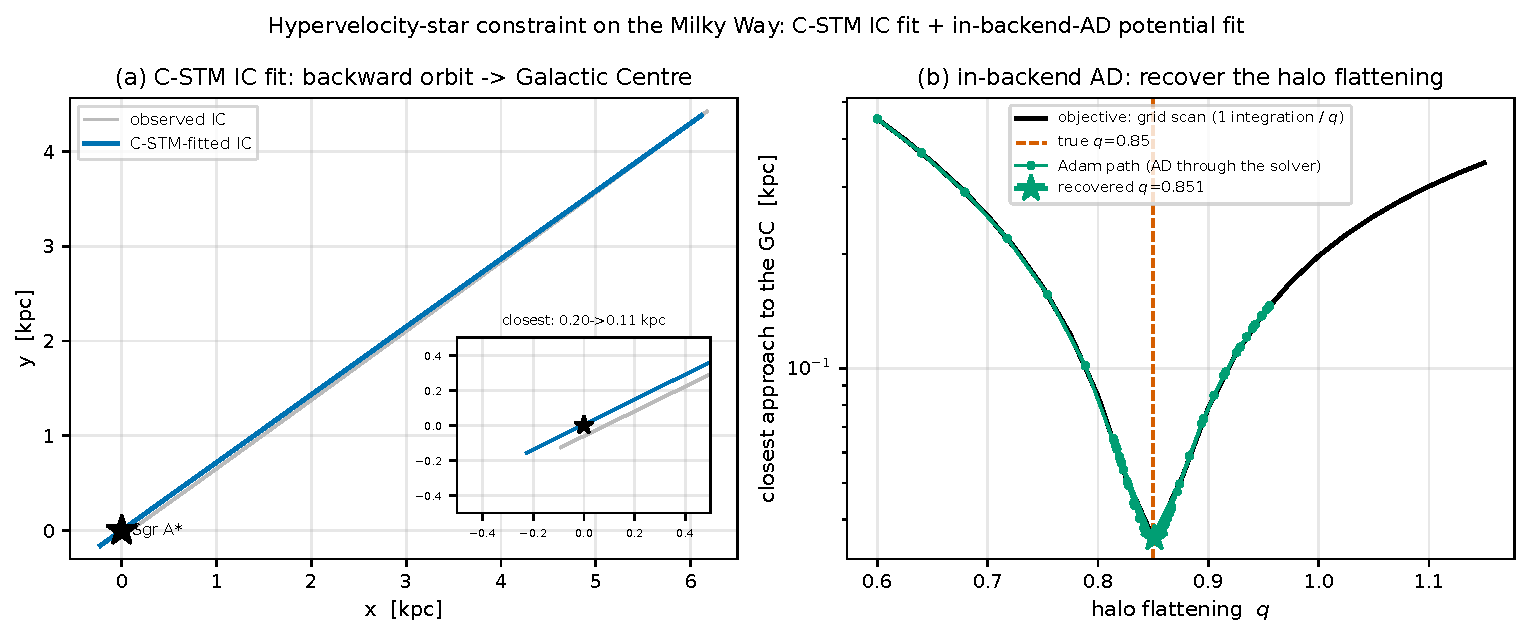
\includegraphics[width=\textwidth,clip=]{../figures/g14_hvs_potential_fit/g14_hvs_potential_fit.pdf}
  \caption{A mock hypervelocity star as a constraint on the Galactic potential.
    Left: the orbit of a star resembling S5-HVS1, integrated backwards
    from its observed phase-space position (grey) and from the position
    within the observational uncertainties that brings the orbit closest
    to Sgr~A$^*$ (blue), found by Gauss--Newton iterations on the
    derivative of the orbit with respect to its initial condition from
    the \cc\ variational integrator. Right: the closest approach to the
    Galactic center of the backward orbit as a function of the
    flattening $q$ of the halo (black, from a grid of integrations) and
    the path of a gradient-descent fit of $q$ using the derivative of the
    closest approach through the in-backend orbit integration (points),
    which recovers the value from which the star was generated (dashed
    line).}\label{fig:hvs}
\end{figure*}

\subsection{Learning the inverse action--angle transformation}\label{sec:examples-neural}

The transformation from actions and angles to positions and velocities
has no closed form in a general potential, and \galpy's implementations
of it are limited to one-dimensional potentials and to the torus
machinery. A differentiable forward transformation makes a different
approach possible: a neural network $G(\vecj,\veca)$ that takes actions
and angles to phase-space positions can be trained by requiring that
\galpy's forward transformation, applied to the network's output,
return the actions and angles that went in. The loss is then a cycle
consistency, $|F(G(\vecj,\veca))-(\vecj,\veca)|^2$, with $F$ the
\texttt{actionAngle} method, and its gradient with respect to the
network's weights flows through $F$. No reference inverse is needed
anywhere in the training. \figurename~\ref{fig:neural} shows this for
the vertical motion in \texttt{MWPotential2014} at the solar radius,
where the exact inverse of \sectionname~\ref{sec:aa-other} exists and
serves as a check, and for the full axisymmetric case with the
St\"{a}ckel approximation, where no reference exists. In the first case a
small network trained in a few minutes, identically under \jax\ and
\torch, reproduces the exact tori to a phase-space error of $0.5$ to
$2\,\%$; in the second, a four-layer network trained for half an hour on
a GPU returns actions on the round trip with a scatter of $7\times10^{-3}$
and reconstructs the meridional orbits that it has never seen. Neither
network is a replacement for a proper inverse, and the point is not the
accuracy of these particular fits but that \galpy's action--angle code
sits inside a training loop, as a layer whose gradient the framework
computes, and that the same code does so in both frameworks.

\begin{figure*}[t!]
  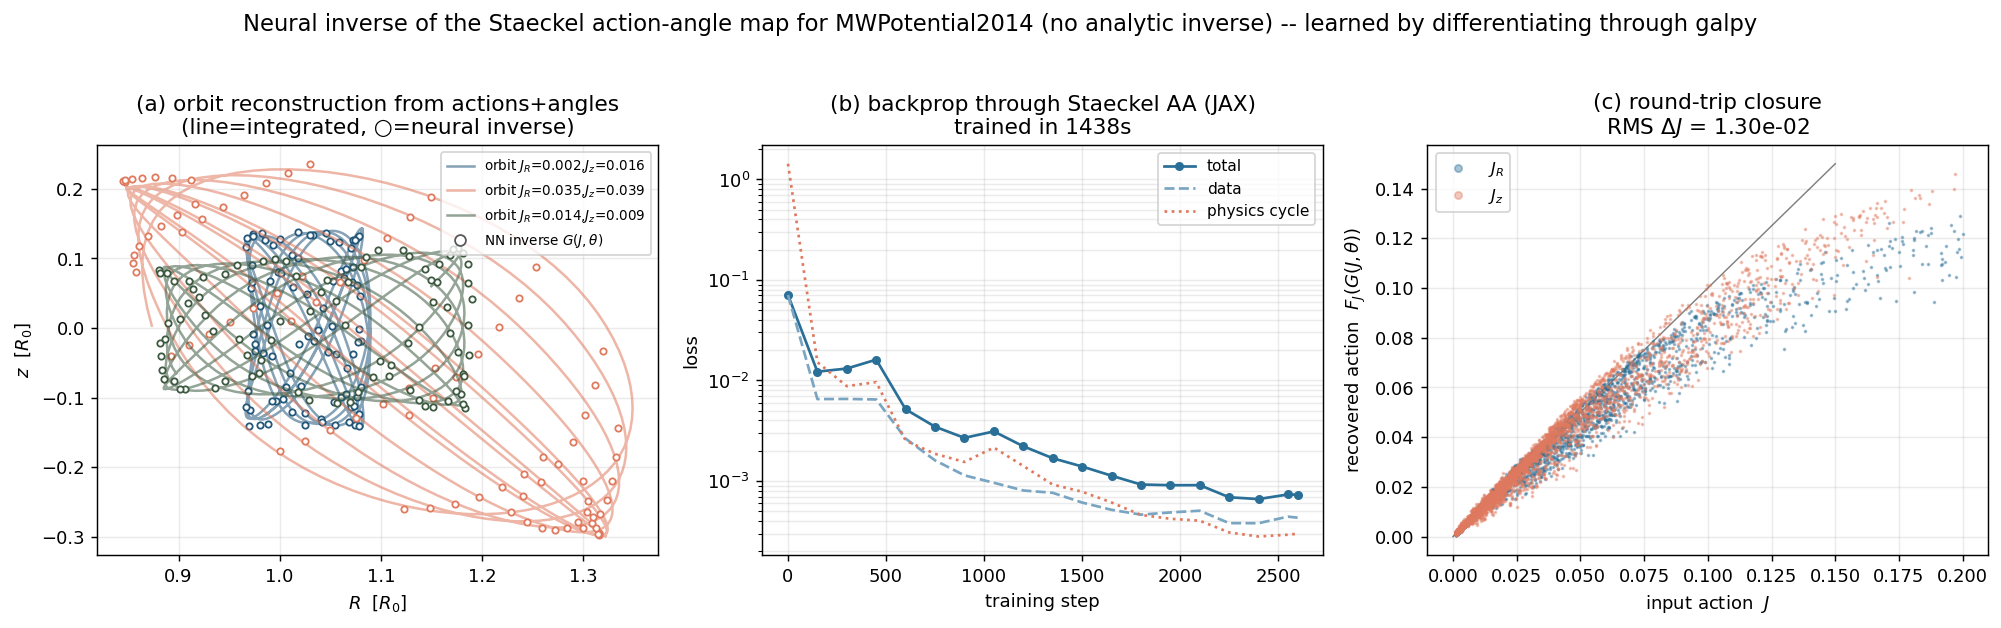
\includegraphics[width=\textwidth,clip=]{../figures/g20_neural_staeckel_inverse/g20_neural_staeckel_inverse.png}
  \caption{Neural inverse of the St\"{a}ckel action--angle transformation
    in \texttt{MWPotential2014} at fixed $L_z$, learned by differentiating
    through \galpy's forward transformation.
    Left: three orbits integrated in the potential (lines) and the
    positions returned by the network for the orbits' actions and
    angles (circles). Middle: the training loss, with its data and
    cycle-consistency terms. Right: the actions recovered by applying
    the forward transformation to the network's output against the
    input actions for a test set.}\label{fig:neural}
\end{figure*}

\section{Conclusion}\label{sec:conclusion}

I have described an extension of \galpy\ that makes it run, compile, and
differentiate under \jax\ and \torch, on CPUs and GPUs, while leaving
its existing \numpy\ and \cc\ implementation byte-for-byte unchanged
and its interface as it was. Potentials, orbit integration, the
action--angle transformations and their inverses, and the distribution
functions, including those of tidal streams, accept the arrays of either
framework and return derivatives with respect to their inputs and
parameters. The existing test suite of \galpy, now 4,275 tests, passes
under \numpy, under both frameworks in eager mode, and under both with
compilation, with six tests remaining as known exceptions, and the
dedicated tests of the backend code add 8,585 more. Derivatives were
tested against finite differences whose convergence is demonstrated,
against the \cc\ variational equations, and against each other across
the two frameworks; where \galpy\ implements a numerical method of its
own, it was tested against \scipy\ and against arbitrary-precision
references. The work also found and fixed about fifty defects in the
\numpy\ and \cc\ code that had been there before.

What this makes possible is the gradient-based fitting of dynamical
models that \galpy\ already contains, with a likelihood whose derivative
with respect to every parameter---of the potential, of the DF, of the
orbits of the objects being modeled---costs a small multiple of the
likelihood itself, and the use of these models as components of larger
differentiable programs, such as neural networks that represent a
potential or a DF, or a simulation whose output is compared with data.
The speed-ups that a GPU provides, of one to three orders of magnitude
for large batches, are a second benefit, and one that depends on
keeping the computation on the device by compiling it as a whole.
Fitting a stream model to data with a Hamiltonian Monte Carlo sampler,
which the derivatives of \sectionname~\ref{sec:streams} allow, is the
obvious next application and will be presented separately.

Some things are not done. The torus-mapping code is not covered and will
not be. \astropy\ units cannot be used inside compiled programs. The
construction of the quasi-isothermal disk DF and of the stream-gap model
are \numpy\ computations, as are the variational equations and Lyapunov
exponents, which are features of the \cc\ integrators. Derivatives
through the \cc\ integrators and the \cc\ action--angle methods are with
respect to the initial conditions only and of first order. And a
backend is a moving target: the special-function fallbacks exist
because the frameworks' own versions are incomplete today, and the test
that checks this will say when they are no longer needed.

The code described here is part of \galpy's main branch from version
\flag{v1.13} on %TODO(JB): version
and is installed with \texttt{pip install galpy[jax]} or
\texttt{galpy[torch]}; the documentation describes the backends at
\\ \centerline{\url{https://docs.galpy.org}~.} All code used to produce
the figures in this paper, together with the working notes and logs of
the development, is available at
\\ \centerline{\url{https://github.com/jobovy/galpy-jax}~.}


\begin{acknowledgments}
It is a pleasure to thank Anthropic for providing a Claude Max
subscription free of charge for the first part of this work, and GitHub
for covering the cost of the continuous integration through its
Education program. We also thank %TODO(JB): people to thank
the many users of \galpy\ whose bug reports and questions over the past
decade shaped the code that is extended here. JB acknowledges financial
support from NSERC (funding reference number RGPIN-2020-04712) and an
Ontario Early Researcher Award (ER16-12-061). %TODO(JB): check current grants
This work was made possible by the open-source codes \numpy\
\citep{Harris2020}, \scipy\ \citep{Virtanen2020}, \matplotlib\
\citep{Hunter2007}, \astropy\ \citep{Astropy2022}, \jax\
\citep{Bradbury2018}, \torch\ \citep{Paszke2019}, \diffrax\ and
\texttt{equinox} \citep{Kidger2021,KidgerGarcia2021}, \texttt{torchdiffeq}
\citep{Chen2018}, \torchode\ \citep{LienenGunnemann2022}, and the GNU Scientific
Library \citep{Galassi2009}. Computations on the H100 GPU were performed
on the Trillium supercomputer at the SciNet HPC Consortium; SciNet is
funded by Innovation, Science and Economic Development Canada, the
Digital Research Alliance of Canada, the Ontario Research Fund: Research
Excellence, and the University of Toronto. %TODO(JB): verify Trillium acknowledgment text
Version-control, continuous-integration, coverage, and documentation
services are provided by GitHub, Codecov, and Read the Docs and are
gratefully acknowledged.
\end{acknowledgments}

\section*{Statement on the use of AI}

This paper has a single human author, JB, but is written in the first
person plural, because the work that it describes was a collaboration
between JB and Claude, an AI coding agent developed by Anthropic and
used through the \texttt{Claude Code} environment. ``We'' refers to that
collaboration; where the distinction matters, as in
\sectionname~\ref{sec:process}, JB and the agent are named separately.
The agent wrote the code described in this paper under JB's direction
and review between 2026 June 1 and October 6; successive
versions of the Claude models were used over this period, and each
commit records the model that produced it. JB set the goals, the
constraints, and the acceptance criteria, reviewed the pull requests,
directed the design where the agent's choices were not what he wanted,
and merged the code; the agent wrote the code, the tests, the
documentation, and the working notes, and ran the measurements. For
about two weeks in the summer the agent worked without supervision, as
described in \sectionname~\ref{sec:process-autonomous}, and JB reviewed
its work from that period afterwards. JB also used OpenAI's Codex to
review the agent's code at several points. The agent produced the figures
of this paper and the analysis behind them from scripts that are part of
the accompanying repository. The text of this paper was
drafted by the agent from the working notes of the project and from JB's
instructions and was then edited by JB, who is responsible for its
content. %TODO(JB): adjust to what actually happened with the text


\appendix
\section{Variational equations and the state-transition matrix}\label{app:dxdv}

This appendix collects the equations behind \texttt{Orbit.integrate\_dxdv},
\texttt{Orbit.lyapunov}, and the derivative rule of the \cc\ integrators
of \sectionname~\ref{sec:orbit-paths}. None of it is specific to a
backend; it is implemented in \cc\ and in \numpy.

Write the phase-space coordinates as $\vecw = (\vecx,\vecv)$ in
rectangular Galactocentric coordinates, in which \galpy's \cc\
integrators work, and the equations of motion as $\dot{\vecw} =
\vec{f}(\vecw,t)$ with $\dot{\vecx} = \vecv$ and $\dot{\vecv} =
\vec{a}(\vecx,\vecv,t)$. A small deviation $\delta\vecw$ from an orbit
evolves according to the linearized equations
\begin{equation}\label{eq:variational}
  \frac{\dd\,\delta\vecw}{\dd t} = \vec{J}(t)\,\delta\vecw\,,\qquad
  \vec{J} = \begin{pmatrix} \vec{0} & \vec{I} \\
    \partial\vec{a}/\partial\vecx & \partial\vec{a}/\partial\vecv\end{pmatrix}\,,
\end{equation}
evaluated along the orbit. For a conservative force,
$\partial\vec{a}/\partial\vecv = \vec{0}$ and $\vec{K} \equiv
\partial\vec{a}/\partial\vecx = -\nabla\nabla\Phi$ is the symmetric
Hessian of the potential. \galpy's potentials provide their second
derivatives in cylindrical coordinates, and $\vec{K}$ is assembled from
them: with $\cos\phi = x/R$ and $\sin\phi = y/R$, the in-plane block is
the one of the planar variational equations that \galpy\ has had since
2011, built from $\partial^2\Phi/\partial R^2$,
$\partial^2\Phi/\partial\phi^2$, and $\partial^2\Phi/\partial R\partial\phi$,
and the vertical couplings are
\begin{align}
  K_{xz} &= -\cos\phi\,\frac{\partial^2\Phi}{\partial R\partial z}
            +\frac{\sin\phi}{R}\,\frac{\partial^2\Phi}{\partial z\partial\phi}\,,\nonumber\\
  K_{yz} &= -\sin\phi\,\frac{\partial^2\Phi}{\partial R\partial z}
            -\frac{\cos\phi}{R}\,\frac{\partial^2\Phi}{\partial z\partial\phi}\,,\\
  K_{zz} &= -\frac{\partial^2\Phi}{\partial z^2}\,.\nonumber
\end{align}
The mixed derivatives $\partial^2\Phi/\partial R\partial z$ and
$\partial^2\Phi/\partial z\partial\phi$ were added to the \cc\ interface
of every potential for this purpose, and the symmetry of $\vec{K}$ is
checked by the test suite. For a dissipative force
$\vec{F}(\vecx,\vecv)$, such as dynamical friction, the lower-right
block $\partial\vec{F}/\partial\vecv$ is non-zero and the lower-left
block is not symmetric; both are implemented for \galpy's
dynamical-friction forces.

The state-transition matrix $\vec{M}(t) = \partial\vecw(t)/\partial\vecw(0)$
is the solution of \eqnname~(\ref{eq:variational}) for six independent
deviation vectors, $\dot{\vec{M}} = \vec{J}\vec{M}$ with
$\vec{M}(0) = \vec{I}$. The Runge--Kutta integrators integrate the orbit
and all six columns as one 42-component state, such that the deviations
see the same steps as the orbit; the symplectic integrators apply to the
deviations the drift ($\delta\vecx \leftarrow \delta\vecx +
h\,\delta\vecv$) and kick ($\delta\vecv \leftarrow \delta\vecv +
h\,\vec{K}\,\delta\vecx$) sub-steps with the same coefficients as the
orbit, which is the tangent map of the integrator and is itself
symplectic. For a conservative force, $\vec{M}$ is symplectic,
$\vec{M}^T\boldsymbol{\Omega}\vec{M} = \boldsymbol{\Omega}$ with
$\boldsymbol{\Omega}$ the standard symplectic form, and in particular
$\det\vec{M} = 1$, which is Liouville's theorem; for a dissipative force,
$\det\vec{M}(t) = \exp\int_0^t \mathrm{tr}\,(\partial\vec{F}/\partial\vecv)\,\dd t'$,
which measures the contraction of phase-space volume. These identities
are necessary but not sufficient checks---a sign error in one block of
$\vec{K}$ can leave the determinant equal to one---and the test that
settles the correctness of $\vec{M}$ is the comparison of its columns
with finite differences of independently integrated orbits, in which the
finite-difference error follows its characteristic V shape with step
size and the variational result sits at the bottom of the V.
\figurename~\ref{fig:variational} shows these checks for a Milky-Way
orbit: the Liouville and symplecticity defects stay below $10^{-6}$ over
a hundred time units, and the state-transition matrix agrees with the
best central difference at the finite-difference floor of $10^{-8}$.

\begin{figure}[t!]
  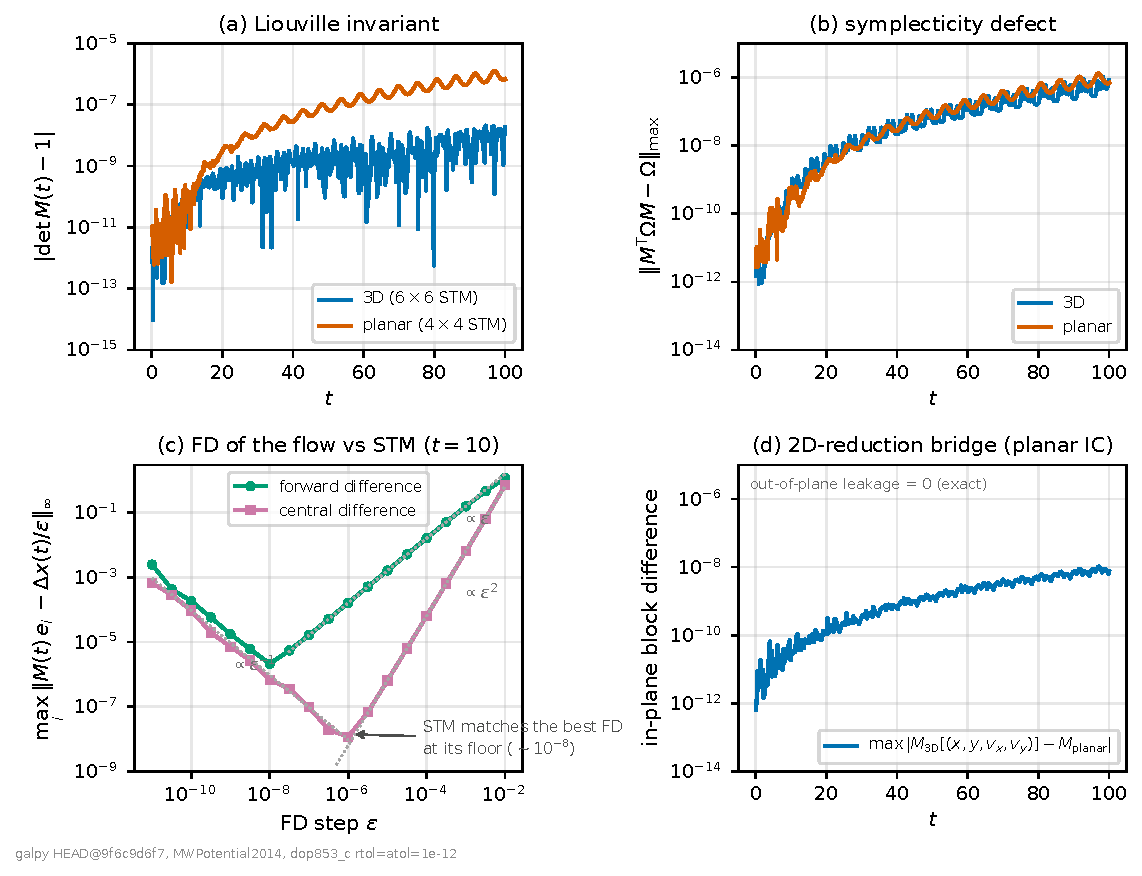
\includegraphics[width=0.48\textwidth,clip=]{../figures/g9_variational_validity/g9_variational_validity.pdf}
  \caption{Checks of the \cc\ variational equations for an orbit in
    \texttt{MWPotential2014}, integrated with \texttt{dop853\_c} at
    tolerances of $10^{-12}$. (a) The Liouville defect $|\det\vec{M}-1|$
    and (b) the symplecticity defect for the three-dimensional and the
    planar state-transition matrix. (c) The difference between the
    columns of $\vec{M}$ at $t=10$ and forward and central finite
    differences of independently integrated orbits as a function of the
    finite-difference step; the variational result agrees with the best
    central difference at its floor. (d) The in-plane block of the
    three-dimensional matrix for a planar initial condition agrees with
    the planar matrix, with no leakage out of the plane.}\label{fig:variational}
\end{figure}

The derivative rule of \sectionname~\ref{sec:orbit-paths} follows from
the chain rule: for a scalar function $L$ of the orbit sampled at times
$t_k$, $\partial L/\partial\vecw(0) = \sum_k \vec{M}(t_k)^T\,
\partial L/\partial\vecw(t_k)$, which is a single matrix--vector product
per output time once $\vec{M}$ is known. Lyapunov exponents are
computed by integrating a deviation vector with
\eqnname~(\ref{eq:variational}), renormalizing it to unit length every
fixed number of steps, and accumulating the logarithms of the
normalization factors \citep{Benettin1980a,Benettin1980b}; the spectrum follows by
orthonormalizing a set of deviation vectors in the same way.


\bibliography{refs}
\bibliographystyle{aasjournalv7}

\end{document}
